\documentclass[10pt,twocolumn,letterpaper]{article}

\usepackage{cvpr}
\usepackage{times}
\usepackage{epsfig}
\usepackage{graphicx}
\usepackage{amsmath}
\usepackage{amssymb}
\usepackage{bbm}

\usepackage[utf8]{inputenc}
\usepackage[english]{babel}
\usepackage[T1]{fontenc}

\usepackage{subcaption}
\usepackage[draft,inline,nomargin]{fixme} % Enable fixme-notes.
\usepackage{units}

\makeatletter
\newcommand*\rel@kern[1]{\kern#1\dimexpr\macc@kerna}
\newcommand*\widebar[1]{%
  \begingroup
  \def\mathaccent##1##2{%
    \rel@kern{0.8}%
    \overline{\rel@kern{-0.8}\macc@nucleus\rel@kern{0.2}}%
    \rel@kern{-0.2}%
  }%
  \macc@depth\@ne
  \let\math@bgroup\@empty \let\math@egroup\macc@set@skewchar
  \mathsurround\z@ \frozen@everymath{\mathgroup\macc@group\relax}%
  \macc@set@skewchar\relax
  \let\mathaccentV\macc@nested@a
  \macc@nested@a\relax111{#1}%
  \endgroup
}
\makeatother

\graphicspath{{pictures/}}

% Include other packages here, before hyperref.

% If you comment hyperref and then uncomment it, you should delete
% egpaper.aux before re-running latex.  (Or just hit 'q' on the first latex
% run, let it finish, and you should be clear).
\usepackage[pagebackref=true,breaklinks=true,letterpaper=true,colorlinks,bookmarks=false]{hyperref}

%\cvprfinalcopy % *** Uncomment this line for the final submission

\def\cvprPaperID{****} % *** Enter the CVPR Paper ID here
\def\httilde{\mbox{\tt\raisebox{-.5ex}{\symbol{126}}}}

% Pages are numbered in submission mode, and unnumbered in camera-ready
\ifcvprfinal\pagestyle{empty}\fi
\begin{document}

%%%%%%%%% TITLE
\title{Tri-modal Human Body Segmentation}

\author{Chris Bahnsen, Andreas Møgelmose, Thomas B. Moeslund\\
Aalborg University\\
Sofiendalsvej 11, 9200 Aalborg SV, Denmark\\
{\tt\small \{cb, am, tbm\}@create.aau.dk}
% For a paper whose authors are all at the same institution,
% omit the following lines up until the closing ``}''.
% Additional authors and addresses can be added with ``\and'',
% just like the second author.
% To save space, use either the email address or home page, not both
}

\maketitle
%\thispagestyle{empty}

%%%%%%%%% ABSTRACT
\begin{abstract}
   The ABSTRACT is to be in fully-justified italicized text, at the top
   of the left-hand column, below the author and affiliation
   information. Use the word ``Abstract'' as the title, in 12-point
   Times, boldface type, centered relative to the column, initially
   capitalized. The abstract is to be in 10-point, single-spaced type.
   Leave two blank lines after the Abstract, then begin the main text.
   Look at previous CVPR abstracts to get a feel for style and length.
\end{abstract}

%%%%%%%%% BODY TEXT
\section{Introduction}
\label{sec:introduction}

Segmentation of people in images is still nowadays a very challenging and tough problem for the computer vision community due to the great diversity of poses that they can adopt and their variable appearance. Difficulties also arise from changes in lighting conditions and complex and cluttered backgrounds. The general idea of human body segmentation is to assign a label to every pixel or group of pixels in an image such that pixels with the same label share certain visual characteristics which entitles them to be considered as part of a human. These type of problems are commonly referred to as labeling problems. Despite extensive research done so far, some constraints have still to be taken into account and one often has to make assumptions about the scenario where the segmentation task is to be applied, such as static versus moving camera, indoor versus outdoor, and so on. Ideally, it should be tackled in an automatic fashion rather than relying on user intervention, which makes such task even more challenging. 

There exist a wide range of possible applications for people segmentation such as surveillance, content-based image retrieval, activity recognition, patient caregiving or human-computer interaction among others. Such task is also often related to pose estimation problems, since it can be carried out efficiently once the person is detected and segmented in an image. Furthermore, it can facilitate the task of photo edition, chroma-keying or video compression. Hence, human body segmentation can be considered as an important preprocessing step for other tasks.

State of the art methods that tackle the human segmentation task mostly use color images recorded by RGB cameras as the main cue for further analysis, although they present several widely known intrinsic problems such as intensity similarities between background and foreground. More recently, the release of RGB-Depth devices such as Microsoft\textsuperscript\textregistered Kinect\textsuperscript\texttrademark , a cheap multi-sensor device based on structured light technology, has allowed the community to use RGB images along with per-pixel depth information, often called depth maps, thus increasing the robustness of the methods. Besides, this device has helped boost research in human pose and behavior analysis.

In this context, we propose adding a third modality: thermal imagery got from thermal infrared cameras, thus complementing other information sources and making easier the segmentation task. Although thermal cameras are relatively expensive devices, their market price is lowering substantially every year --as it happens with other sensory devices. Besides, they can capture data similar to standard color cameras but without having illumination problems, that is why infrared cameras are becoming popular in surveillance scenarios and other similar applications. To do so, we introduce a novel tri-modal database provided by researchers from Aalborg University in Denmark and Universitat de Barcelona. Such database contains people acting in three different video sequences, consisting of more than 2,000 frames each one, in which three different subjects appear and interact with objects performing diverse actions such as reading, working with a laptop, speaking on the phone, etc. There may be more than one subject appearing in scene. The dataset comes along with an algorithm that performs the registration among modalities. 

In addition, we present a baseline methodology to automatically segment people in video sequences in indoor scenarios with a fixed camera. With all the available modalities, important features will be extracted using different state of the art descriptors, which are used to learn a probabilistic model so as to predict the image regions belonging to people. We will compare results from applying segmentation to the different modalities separately to results obtained by fusing features from all modalities.

To the best of our knowledge, this is the first dataset and work that combines color, depth and thermal modalities to perform the people segmentation task in videos, aiming to bring further benefits towards developing more robust solutions.

The remainder of this dissertation is organized as follows. Section \ref{sec:relatedwork} reviews the different approaches for human body segmentation that appear in the recent literature. Section \ref{sec:trimodalhumanbodysegmentation} introduces and exhaustively explains the proposed baseline methodology, which will be experimentally evaluated in Section \ref{sec:evaluation}. Finally, Section \ref{sec:conclusions} concludes this dissertation.

\section{Related work}
\label{sec:relatedwork}

Image segmentation is one of the oldest and most widely studied problems in computer vision \cite{brice1970scene, riseman1977computational, ohlander1978picture, rosenfeld1979image, haralick1985image}. First approaches had a tendency to use region splitting or merging, which correspond to divisive and agglomerative clustering respectively. Later, research focused on methods that try to optimize some criteria, such as inter-region boundary lengths, intra-region consistency or dissimilarity \cite{szeliski2011computer}. Due to the vast work available on image segmentation, in this section we are going to focus in the most recent and relevant works, techniques and methods applied specifically to human body segmentation that determine the state of the art.

\subsection{Methods}
Within the last decade a great number of novel approaches have emerged to respond to different requirements in the human segmentation context, such as trying to overcome changing illumination conditions, dealing with variable human poses or developing quasi-automatic systems that progressively lose the need for user intervention.
 
 When dealing with indoor scenarios recorded by a stationary camera, the pixel-based background subtraction approach can be applied successfully. We can model the background distribution of the scene and detect moving objects by comparing each pixel to the model, which are considered as foreground. The result is a silhouette of the moving object, which can be further used for other tasks. Pixel intensity is the most commonly used feature in background modeling, though there are many approaches that use other type of information such as edge, motion, stereo or texture features. The parametric model that Stauffer and Grimson proposed in \cite{stauffer1999adaptive}, which models the background using a mixture of gaussians (MoG), has been widely used and many variations have been suggested based on it. In \cite{bouwmans2011recent}, more advanced statistical background modeling techniques are deeply reviewed. 
 
Nonetheless, after obtaining the moving object contours we still need a way to assess whether they belong to a human or not. Human detection methods are strongly related to the task of human body segmentation since they allow to discriminate better between other objects. They usually produce a bounding box indicating where the person is, which in turn may be also useful as a prior for pixel-based or bottom-up approaches to refine the final human body silhouette. In the category of holistic body detectors, one of the most successful representations is the Histogram of Oriented Gradients (HOG) \cite{dalal2005histograms}, still being the basis of many current detectors. Used along with a discriminative classifier --e.g. Support Vector Machines (SVM) \cite{hearst1998support} --it is able to accurately predict the presence of human subjects. Example-based methods \cite{andriluka2010monocular} have been also proposed to address human detection, utilizing templates to compare the incoming image and locate the person, limiting the pose variability though.  

Regarding descriptors, other possible representations apart from the already commented HOG are those that try to fit the human body into silhouettes \cite{mittal2003human}, those that model color or texture such as Haar-like wavelets \cite{viola2005detecting}, optical flow quantized in Histrograms of Optical Flow (HOOF) \cite{dalal2006human}, depth maps \cite{plagemann2010real} and, more recently, descriptors including logical relations, e.g. Grouplets \cite{yao2010grouplet}, which enables to recognize human-object interactions.

Instead of whole body detection, some approaches have been built under the assumption that the human body consists of an ensemble of body parts \cite{ramanan2006learning, pirsiavash2012steerable}. Some of them are based on pictorial structures \cite{andriluka2009pictorial, yang2011articulated}. In particular, \cite{yang2011articulated, yang2012articulated} from Yang and Ramanan along with \cite{felzenszwalb2010object} from Felzenszwalb have outperformed other existing methods using a Deformable Part-based Model (DPM) that consists on a root HOG-like filter and different part-filters that define a score map of an object hyphotesis, using latent SVM as a classifier. Another well-known part-based detector is Poselets \cite{bourdev2009poselets, wang2011learning}, which trains different homonymous parts to fire at a given part of the object at a given pose and viewpoint. Grammar models \cite{girshick2011object} and AND-OR graphs \cite{zhu2008max} have been also used in this context.


By the same token, other approaches model objects as an ensemble of local features. In this category there are included methods such as Implicit Shape Models (ISM) \cite{leibe2004combined}, consisting of visual words combined with location information. In addition, they are used in works that estimate the class-specific segmentation based on the detection result after a training stage \cite{leibe2008robust}.  

Conversely, generative classifiers directly deal with the person segmentation problem. They function in a bottom-up manner, learning a model from a initial prior in the form of bounding boxes or seeds, and using it to yield an estimate for the background and target distributions, normally applying Expectation Maximization (EM) \cite{shi2000normalized, carson2002blobworld}. One of the most popular is GrabCut \cite{rother2004grabcut}, an interactive segmentation method based on graph cuts \cite{boykov2001interactive} and Conditional Random Fields (CRF) that, using a bounding box as an initialization region, combines pixel appearance information with neighborhood relations to refine silhouettes up to a very accurate level. Graph cuts method has been further applied to part-based approaches \cite{hernandez2012graph}.
%When the scenario is static camera sequences are used, pixel-based approaches play an important role 
 % It is robust to illumination and local contrast changes and scale invariant. 
 
Having considered the properties of each one of the aforementioned segmentation categories, it is reasonable that several approaches have been proposed towards their combination, that is, top-down and bottom-up segmentation \cite{lin2007interactive, mori2004recovering, ladicky2010and, levin2006learning}. Just to name a few, ObjCut \cite{kumar2005obj} combines pictorial structures and Markov Random Fields (MRF) to obtain the final segmentation. PoseCut \cite{bray2006posecut} is also based on MRF and graph cuts but it has the added ability to deal with 3-D pose estimation from multiple views.
 
According to the nature of our proposal, we find appropriate to dedicate a few lines regarding thermal imagery and associated descriptors. In contrast to color or depth cues, thermal infrared imagery has not been used that widely for human detection and segmentation purposes, although it is experiencing a growing interest by the research community. Several specific descriptors have been proposed so far. For example, in \cite{zhang2007pedestrian}, the authors extended the combination of edgelets and HOG features with AdaBoost and SVM cascade to infrared images. Background subtraction has been also adapted to deal with this kind of imagery in \cite{davis2004robust}, which presented a statistical contour-based technique that eliminates typical halo artifacts produced by infrared sensors by combine foreground and background gradient information into a contour saliency map so as to find the strongest salient contours. More recently, \cite{mogelmosetri} presented a person re-identification method that for the first time combined RGB, depth, and thermal features. An extensive survey of thermal cameras and their applications can be found in \cite{gade2014thermal}, including technological aspects and the nature of thermal radiation. 
 
 \begin{figure}
	 \centering
	 \begin{subfigure}[b]{0.25\textwidth}
 		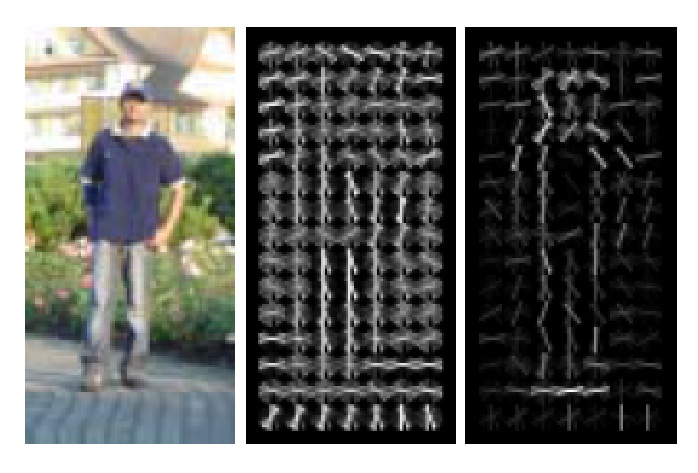
\includegraphics[width=1\textwidth]{pictures/stateoftheart/hog.eps}
 		\caption{}
    		\label{fig:soa_hog}
 	\end{subfigure}
	 ~
	\begin{subfigure}[b]{0.22\textwidth}
 		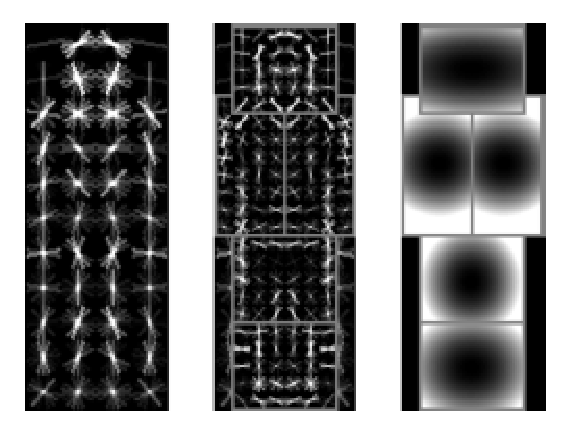
\includegraphics[width=1\textwidth]{pictures/stateoftheart/felzenszwalb2010object.eps}
 		\caption{}
    		\label{fig:soa_dpm}
 	\end{subfigure}
	 ~
	\begin{subfigure}[b]{0.42\textwidth}
 		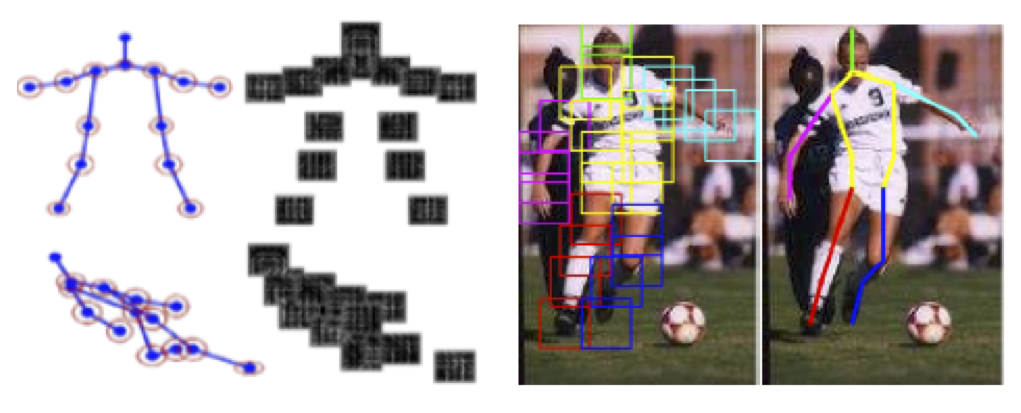
\includegraphics[width=1\textwidth]{pictures/stateoftheart/yang2012articulated.eps} 			
		\caption{}
    		\label{fig:soa_mop}
 	\end{subfigure}
	\\
%	\begin{subfigure}[b]{0.6\textwidth}
% 		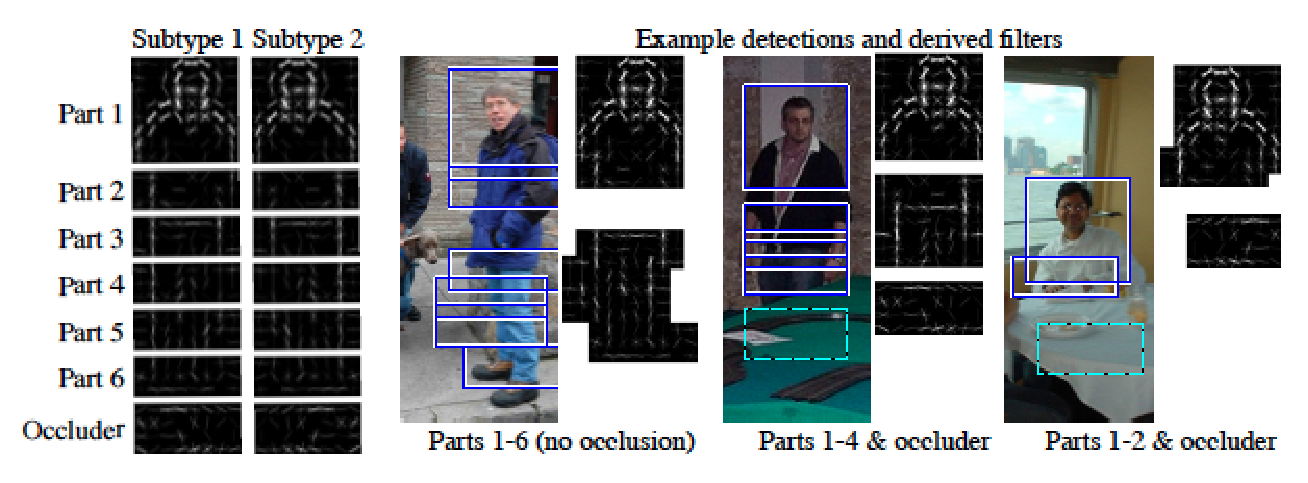
\includegraphics[width=1\textwidth]{pictures/stateoftheart/girshick2011object.eps} 			
%		\caption{}
%    		\label{fig:gull}
% 	\end{subfigure}
%	~
	\begin{subfigure}[b]{0.4\textwidth}
 		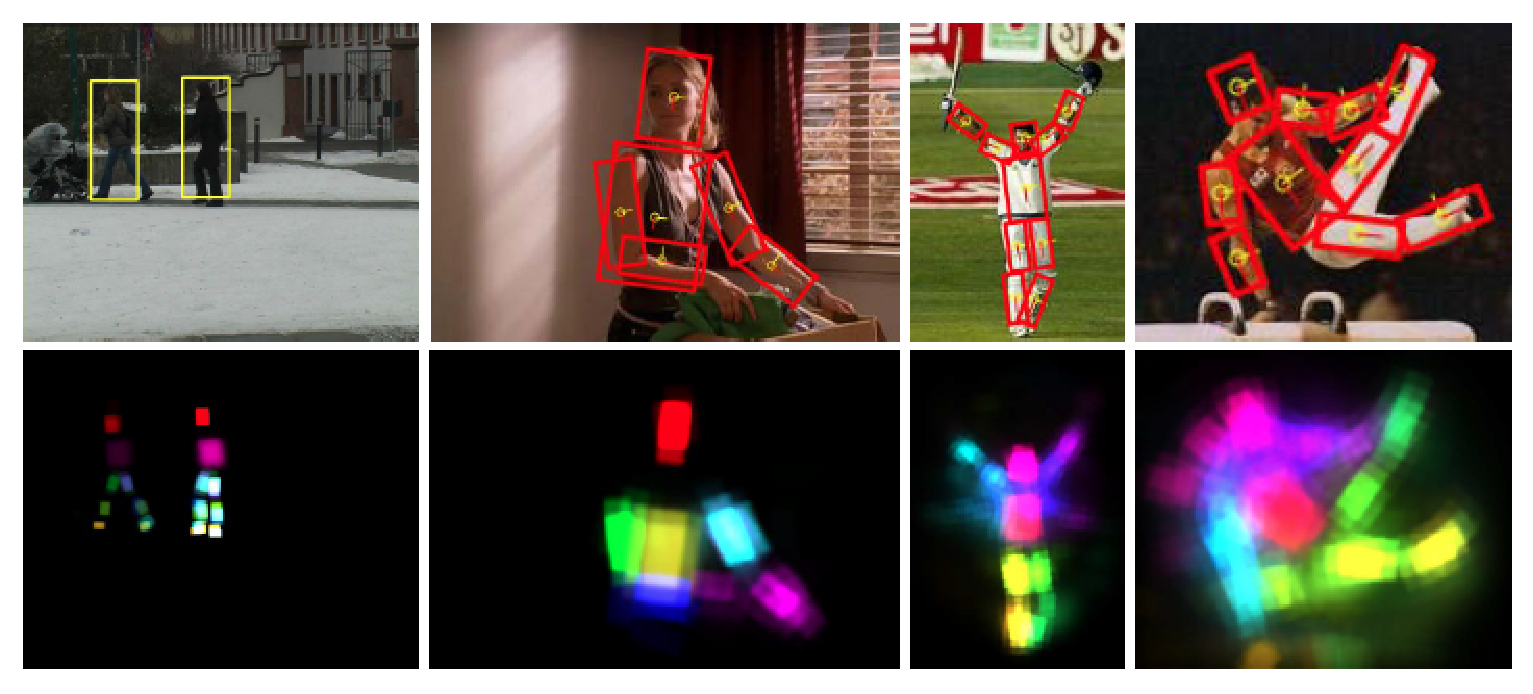
\includegraphics[width=1\textwidth]{pictures/stateoftheart/andriluka2009pictorial.eps} 			
		\caption{}
    		\label{fig:soa_ps}
 	\end{subfigure}
	~
	\begin{subfigure}[b]{0.55\textwidth}
 		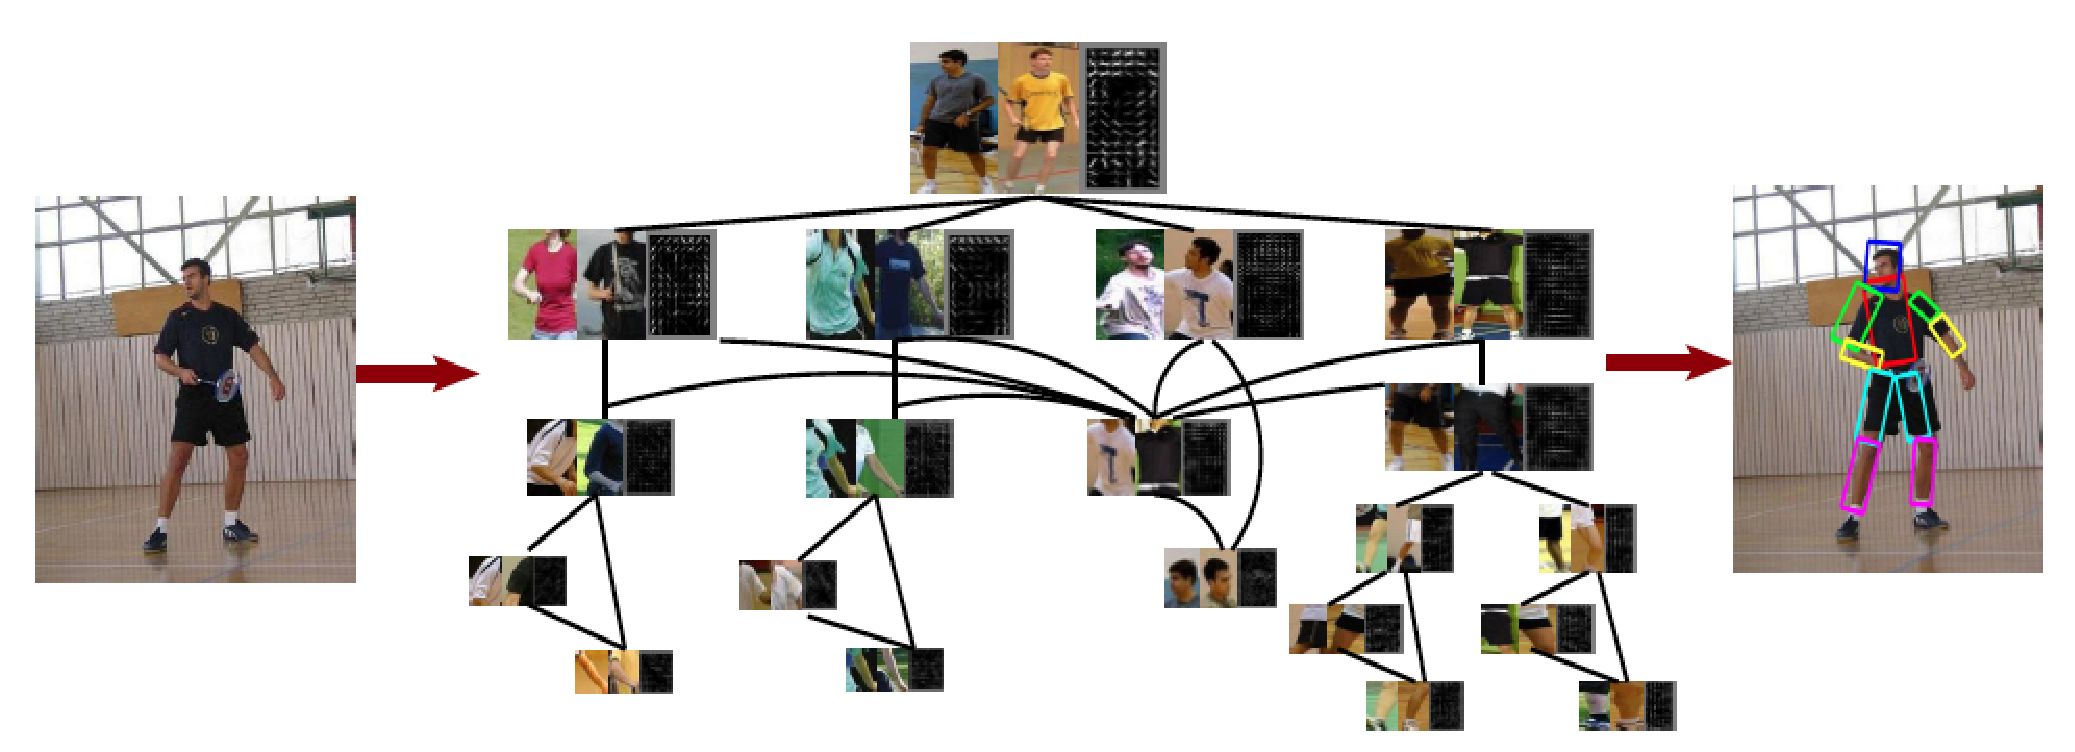
\includegraphics[width=1\textwidth]{pictures/stateoftheart/wang2011learning.eps} 			
		\caption{}
    		\label{fig:soa_poselets}
 	\end{subfigure}
	\\
	\begin{subfigure}[b]{0.45\textwidth}
 		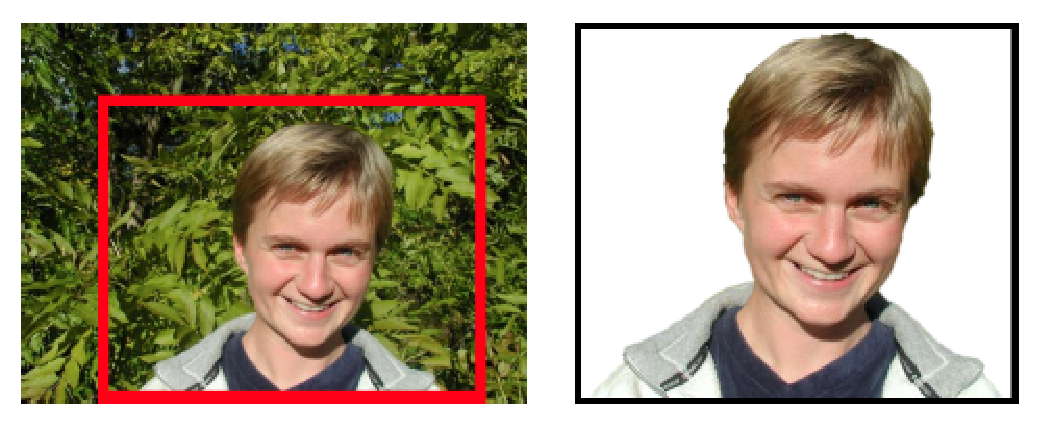
\includegraphics[width=1\textwidth]{pictures/stateoftheart/grabcut.eps} 			
		\caption{}
    		\label{fig:soa_grabcut}
 	\end{subfigure}
	~
	\begin{subfigure}[b]{0.49\textwidth}
 		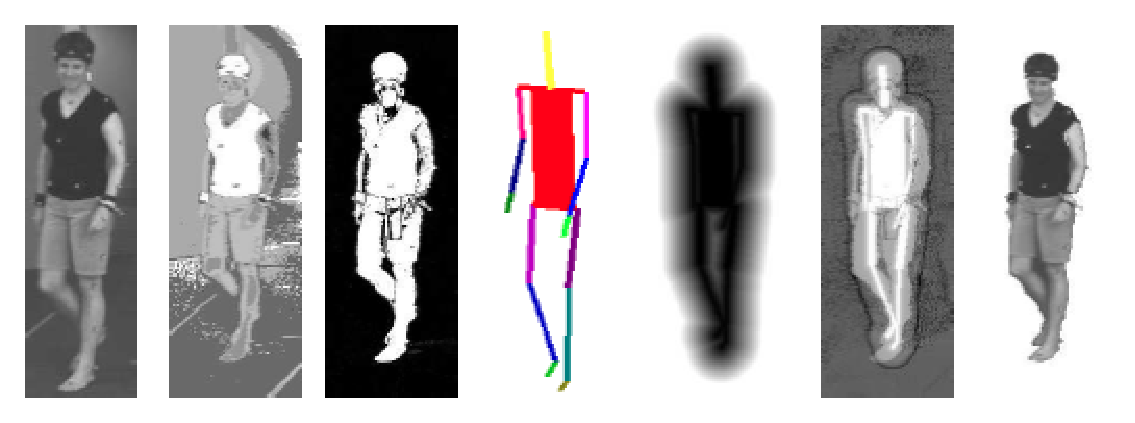
\includegraphics[width=1\textwidth]{pictures/stateoftheart/bray2006posecut.eps} 			
		\caption{}
    		\label{fig:soa_posecut}
 	\end{subfigure}
	\\
 	\begin{subfigure}[b]{1\textwidth}
 		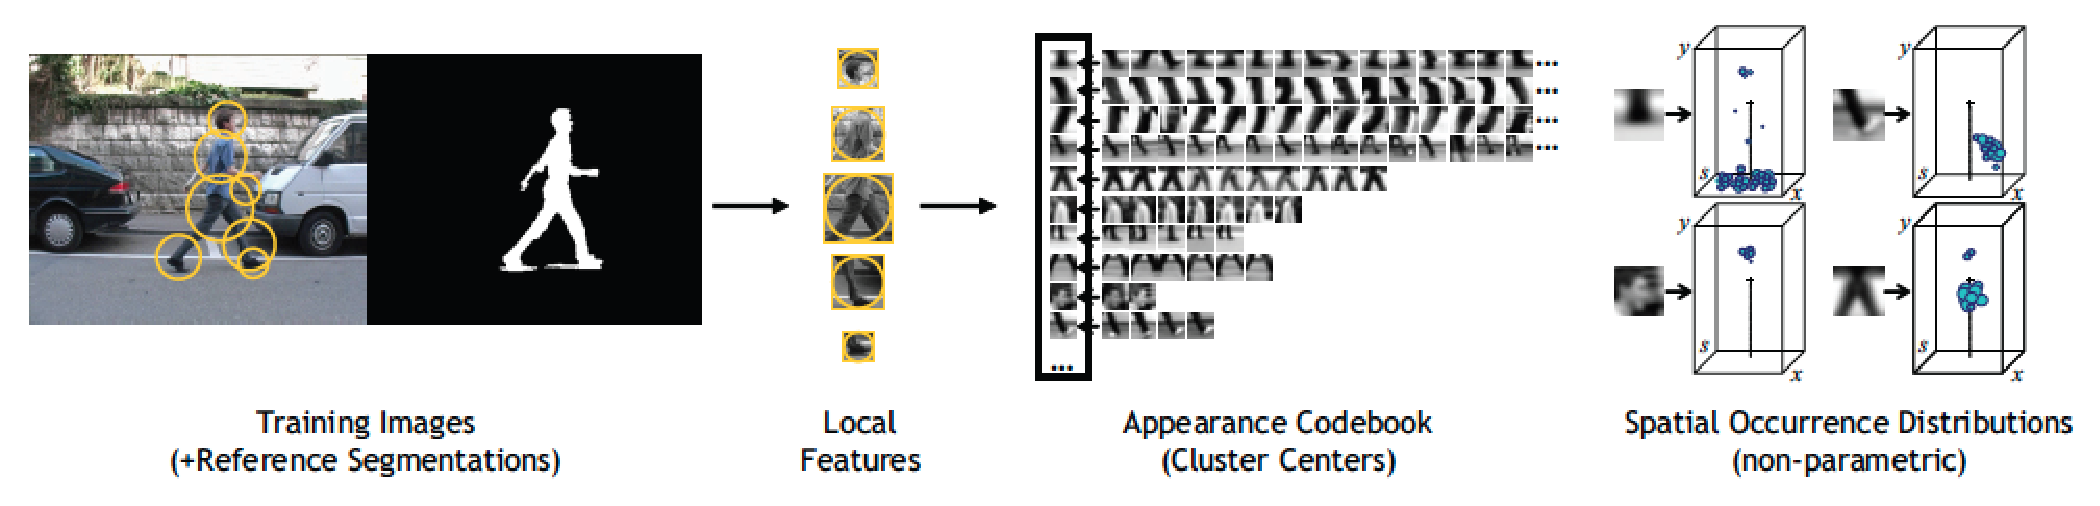
\includegraphics[width=1\textwidth]{pictures/stateoftheart/leibe2008robust.eps}
 		\caption{}
    		\label{fig:soa_ism}
 	\end{subfigure}
 	\\
  	\begin{subfigure}[b]{1\textwidth}
		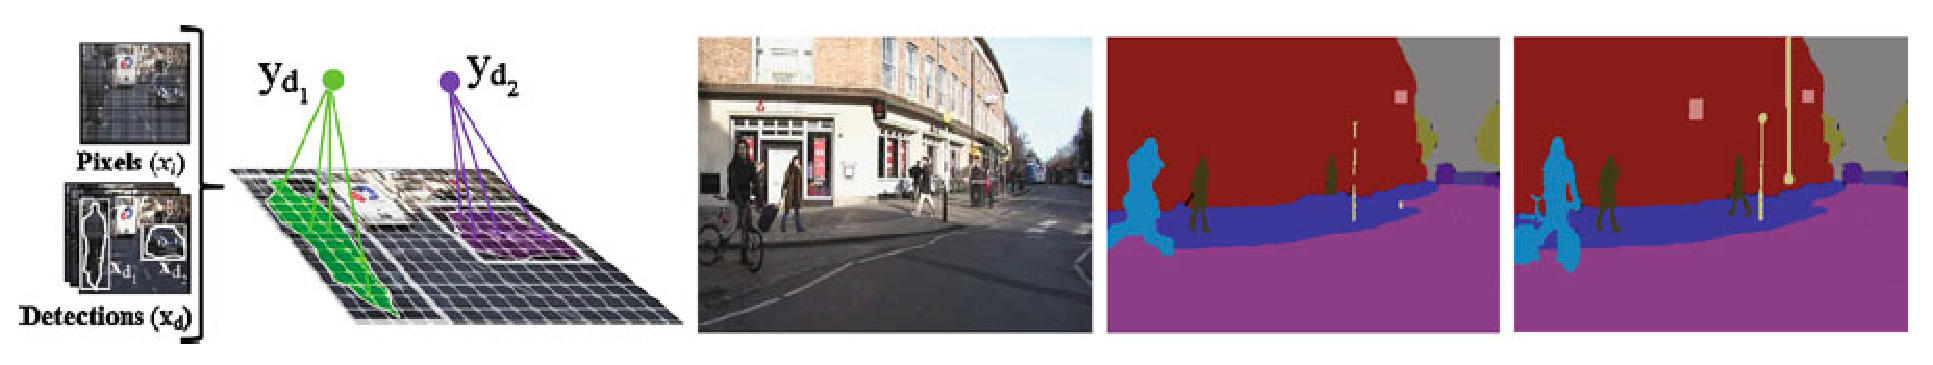
\includegraphics[width=1\textwidth]{pictures/stateoftheart/ladicky2010and.eps}
 		%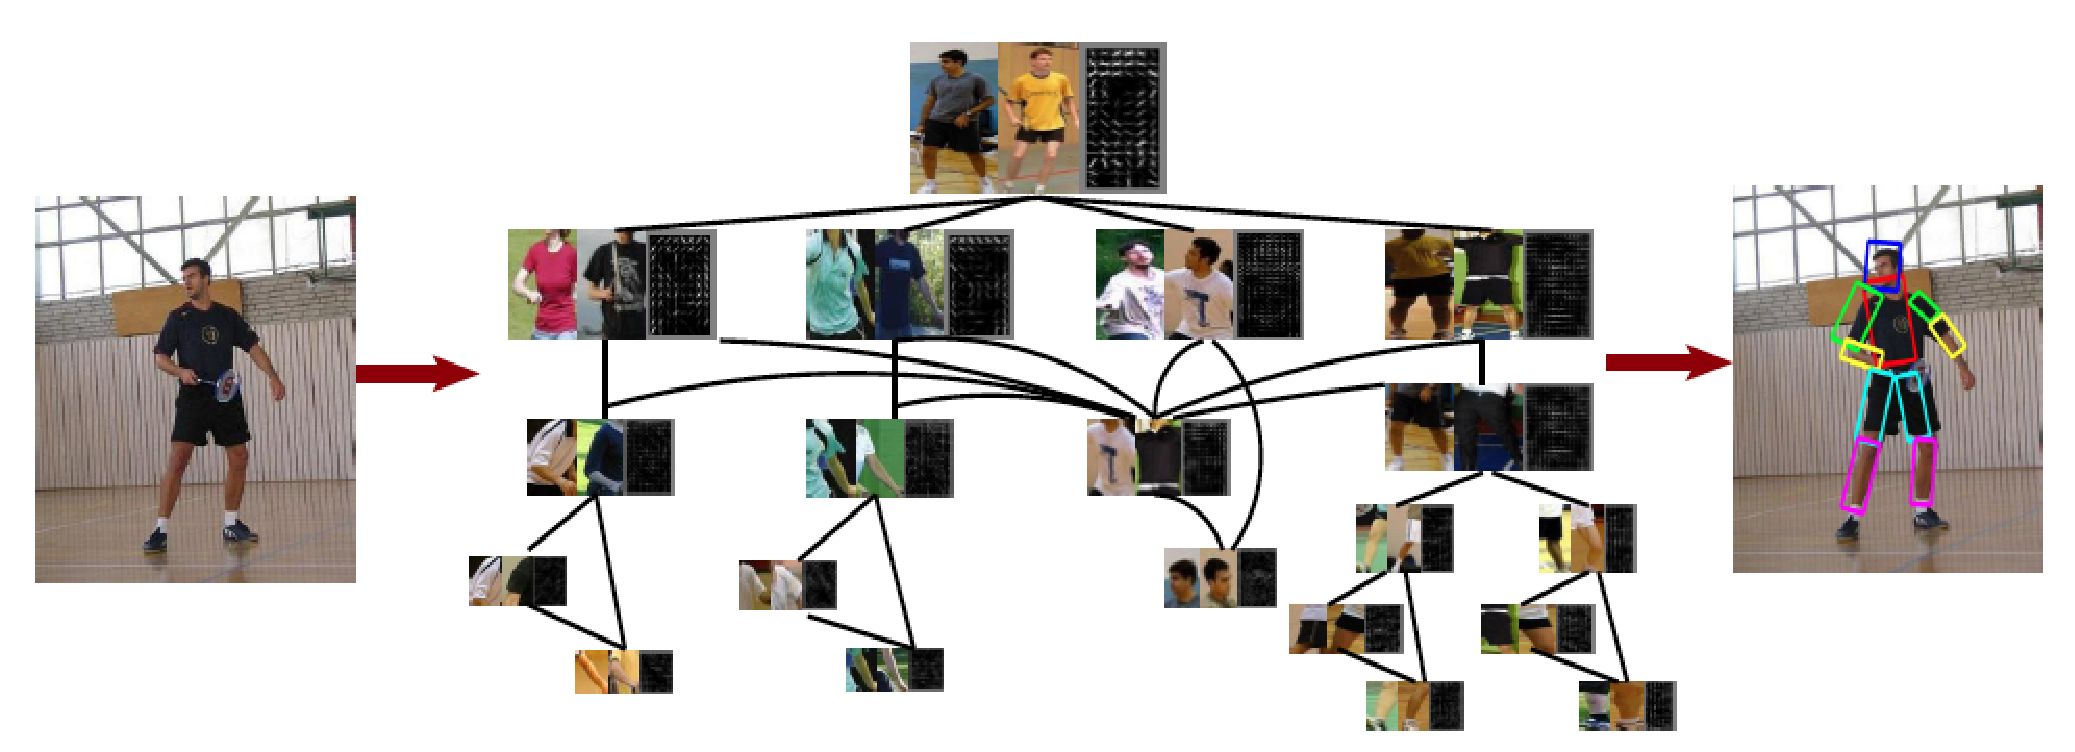
\includegraphics[width=\textwidth]{pictures/stateoftheart/wang2011learning.eps}
 		\caption{}
         	\label{fig:soa_crf}
 	\end{subfigure}
% 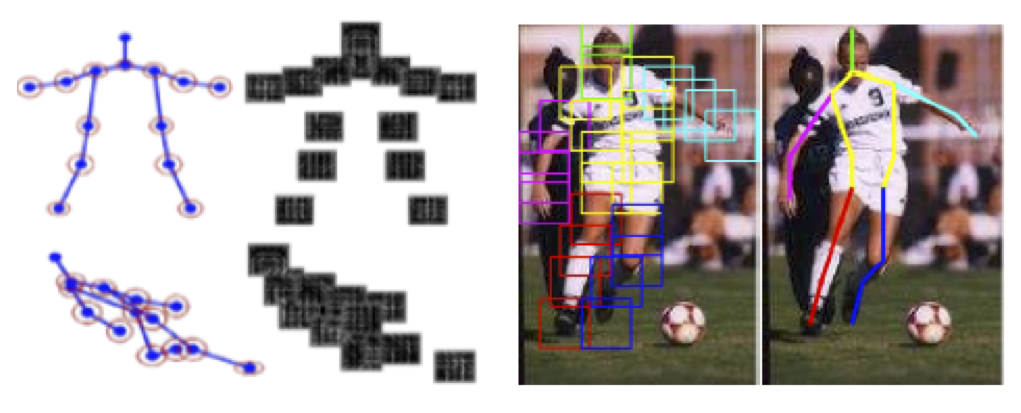
\includegraphics[width=1\textwidth]{pictures/stateoftheart/yang2012articulated.eps}
 	\caption{Examples of recent methods and descriptors: (A) HOG \cite{dalal2005histograms}: Person and his computed HOG descriptor, and the descriptor weighted by positive SVM weights; (B) Deformable Part-based Model \cite{felzenszwalb2010object}: coarse root filter, spatial model for the location of each part and cost of placing the center of a part at different locations relative to the root, respectively; (C) Mixture of parts from \cite{yang2012articulated}: different trees obtained from the mixture of parts and estimation of parts and pose; (D) Pictorial structures \cite{andriluka2009pictorial}: pedestrian detection and upper-body and full body pose estimations, respectively; (E) Poselets \cite{wang2011learning}: each part shows its inferred poselet and the SVM HOG template; (F) GrabCut \cite{rother2004grabcut}: rectangle defined by the user that acts as a bounding box prior and object extracted based on it; (G) PoseCut \cite{bray2006posecut} in order of appearance: original image, pixel likelihood for being labeled as foreground or background, segmentation after using the GMM models, optimal estimated pose, shape prior corresponding to the optimal pose, likelihood after fusing the previous information, and final segmentation; (H) ISM for segmentation \cite{leibe2008robust}: training procedure, where local features are extracted from interest points and clustered to create an appearance codebook, which allows to learn a spatial occurrence distribution for each entry; (I) bottom-up top-down segmentation \cite{ladicky2010and}: CRF structure, original image, and results before and after applying GrabCut to each detected bounding box, respectively.}
 	\label{fig:stateoftheartmethods}
\end{figure}
 
\subsection{Benchmark datasets}
 
To advance research in this area, it is a must to have the right means to compare existent methods so as to allow improvements to be measured. It is not easy to find large image segmentation databases due to the tedious task that manual labeling implies. In this context, the appearance of crowdsourcing-based frameworks such as Amazon Mechanical Turk \cite{mechanicalturk} or LabelMe \cite{russell2008labelme} has encouraged users to participate in with little easy tasks such as image segmentation or annotation, thus gamificating somehow the laborious task of human-labeling and helping the computer vision community to obtain ground truth information at a lower cost.  

Either way, there exist several static image-based human-labeled databases, which allow us to compare the great deal of available literature of image segmentation. The best known of these is the Berkeley Segmentation Dataset and Benchmark\footnote{\url{http://www.eecs.berkeley.edu/Research/Projects/CS/vision/grouping/segbench/}} \cite{martin2001database}, which consists of 12,000 segmentations of 1,000 Corel dataset color images, containing people or different objects. It also includes figure-ground labelings for a subset of the images. Authors of \cite{alpert2007} made also available a database\footnote{\url{http://www.wisdom.weizmann.ac.il/\%7Evision/Seg_Evaluation_DB/index.html}} containing 200 gray level images along with ground truth segmentations, which was specially designed to avoid potential ambiguities by only incorporating images that clearly depict one or two objects in the foreground that differ from its surroundings by either texture, intensity, or other low level cues, but it does not represent uncontrolled scenarios. The well known PASCAL Visual Object Classes Challenge \cite{everingham2012pascal} tended to include a subset of the color images annotated in a pixel-wise fashion for the segmentation competition. Although not considered to be benchmarks, Kinect-based datasets are also available, since this device is being widely used in human pose related works. In \cite{gulshan2011humanising} a novel dataset\footnote{\url{http://www.robots.ox.ac.uk/~vgg/data/humanSeg/}} was presented, which contains 3,386 images of segmented humans and ground truth automatically created by Kinect, and consisting of different human subjects across 4 different locations. Unfortunately, depth map images are not included in the public dataset. 

However, there is a lack of a standard database of videos that can be used for evaluation purposes, such as visual surveillance approaches. There exist some popular ones which try to provide realistic settings and environmental conditions \cite{moeslund2011visual}. Among all of them, we underline the collective datasets of Project ETISEO\footnote{\url{http://www-sop.inria.fr/orion/ETISEO/download.htm}} \cite{nghiem2007etiseo}, owing to the fact that for some of the scenes the authors include, apart from color images, an additional imaging modality such as infrared footage. It consists of indoor and outdoor scenes of public places such as an airport apron or a subway station, and also includes a frame-based annotated ground truth. Depth modality is used in some works such as the RGB-D People Dataset\footnote{\url{http://www.informatik.uni-freiburg.de/~spinello/RGBD-dataset.html}} \cite{spinello2011people}, which presented a dataset containing more than 3,000 RGB-Depth frames using Kinect. The sequences show mostly upright walking and standing persons from a range of orientations and different levels of occlusions, although the annotation is done in a bounding-box fashion, that is, only detecting people.



\section{Acquisition}
\label{sec:setup}
The tri-modal data stream is recorded using a Microsoft Kinect for XBOX 360 capturing the RGB and depth image streams, and an AXIS Q1922 thermal camera. The resolution of the imagery is fixed at 640x480 pixels. As seen in Figure \ref{fig:camerasetup}, the cameras are vertically aligned in order to reduce perspective distortion. 

\begin{figure}[htpb]
	\centering
		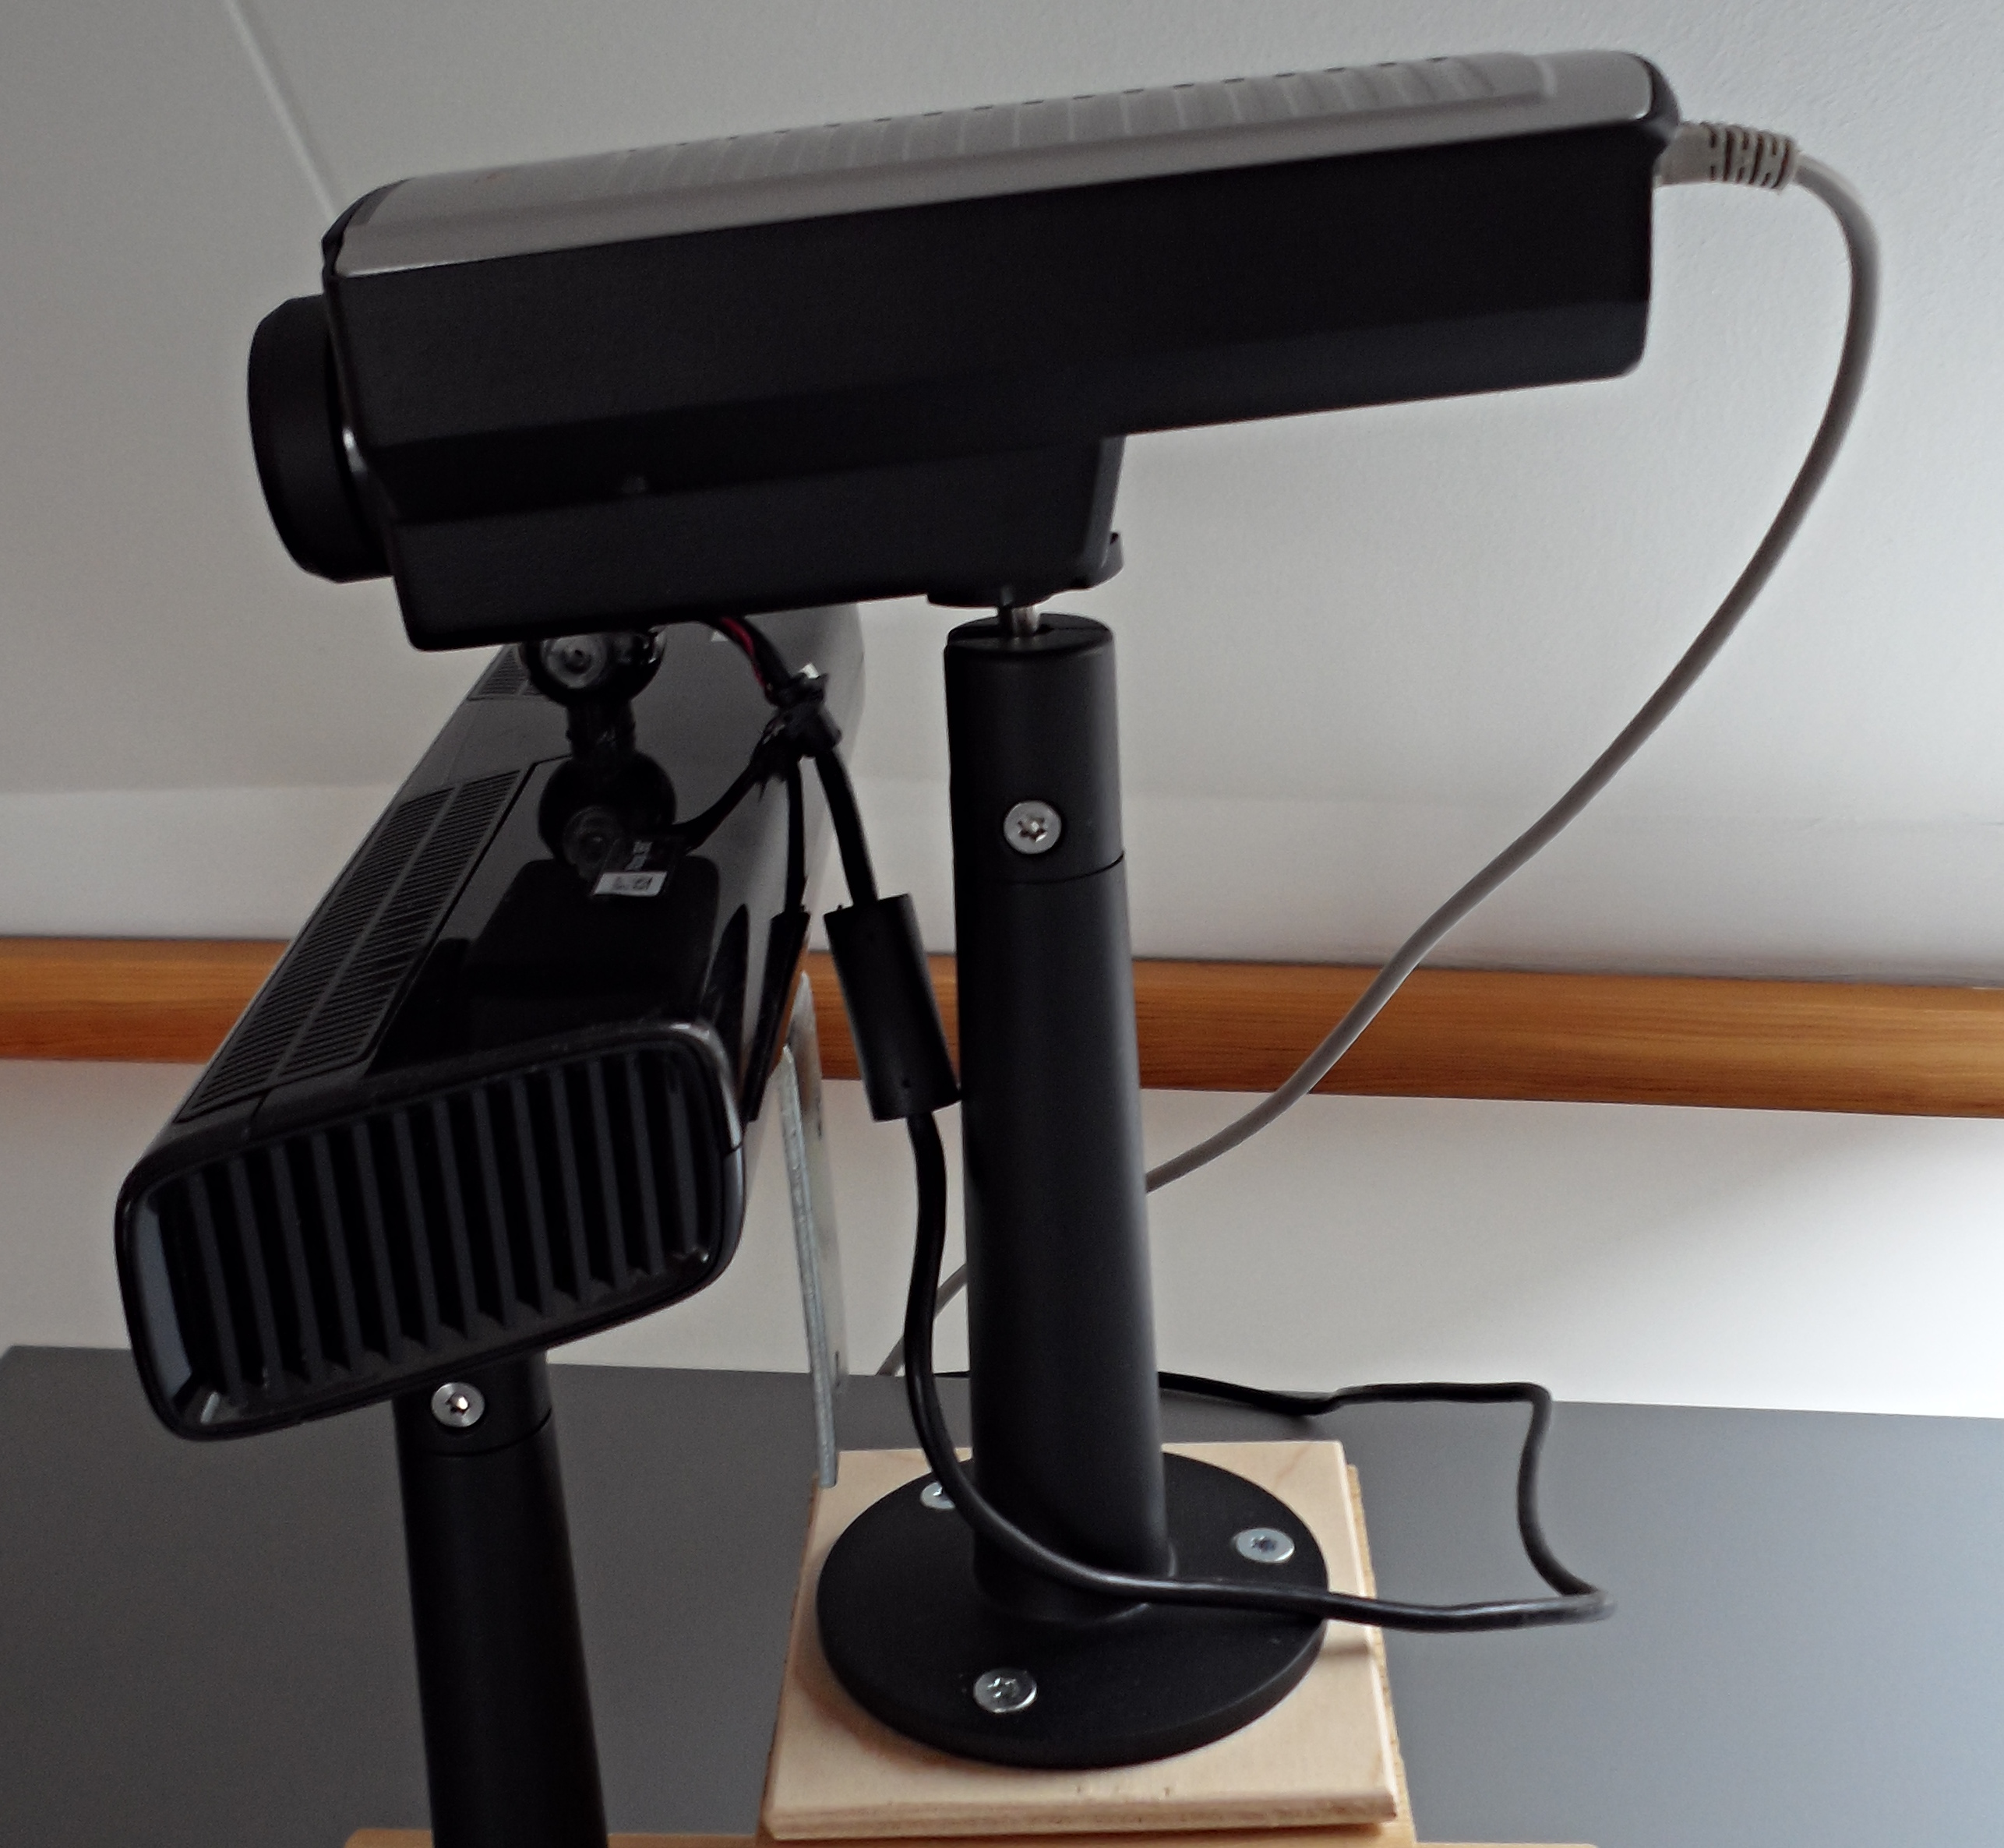
\includegraphics[width=0.25\textwidth]{pictures/camerasetup.jpg}
	\caption{Camera configuration. The RGB and thermal sensor are vertically aligned.}
	\label{fig:camerasetup}
\end{figure}

The image streams are captured using custom recording software that invokes the Kinect for Windows and AXIS Media Control SDKs. The integration of the two SDKs enables the cameras to be calibrated against the same system clock, which enables the post-capture temporal alignment of the image streams. Both cameras are able to record at 30 FPS. However, the data set is recorded at 15 FPS due to performance constraints of the recording software. 

\subsection{Multi-modal calibration}
The calibration of the thermal and RGB cameras have been accomplished using a thermal-visible calibration device inspired by \cite{vidas2012mask}. The calibration device consists of two parts; an A3-sized 10 mm polystyrene foam board is used as a backdrop and an equally sized board with cut-out squares is used as the checkerboard. Before using the calibration device, the backdrop is heated and the checkerboard plate is kept at room temperature, thus keeping a suitable thermal contrast when joined, as is seen from Figure \ref{fig:calibrationDevice}. %The depth sensor of the Kinect is factory calibrated and a subsequent calibration is thus not needed.
Using the Camera Calibration Toolbox of \cite{bouguet2004camera}, we are able to extract corresponding points in the thermal and RGB modalities. The sets of corresponding points are used to undistort both image streams and for the subsequent registration of the modalities. 

\begin{figure}[htpb]
\centering
\begin{subfigure}[b]{0.48\columnwidth}
	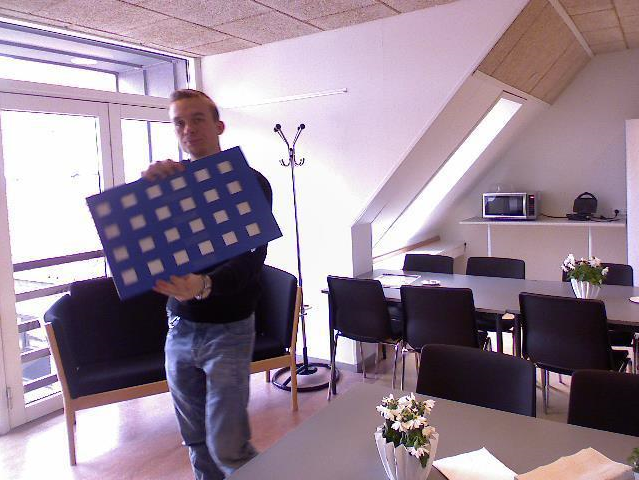
\includegraphics[width=\columnwidth]{RGB00064.png}%
	\caption{}
\end{subfigure}
\begin{subfigure}[b]{0.48\columnwidth}
	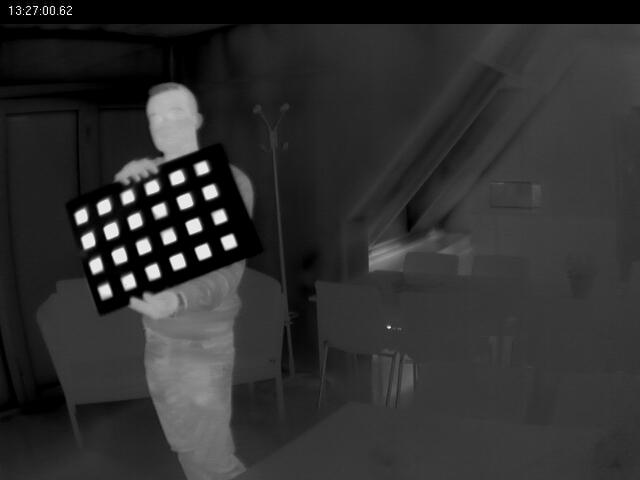
\includegraphics[width=\columnwidth]{T00064.jpg}%
	\caption{}%
\end{subfigure}
\begin{subfigure}[b]{0.48\columnwidth}
	\includegraphics[width=\columnwidth]{plane1.pdf}%
	\caption{}
\end{subfigure}
\begin{subfigure}[b]{0.48\columnwidth}
	\includegraphics[width=\columnwidth]{plane3.pdf}%
	\caption{}%
\end{subfigure}
\caption{The calibration device as seen by the (a) RGB and (b) thermal camera. The corresponding points in world coordinates is seen in (c) and the plane, which induces an homography, is overlayed in (d). Noise in the depth information accounts for the outliers in (c) and (d).}
\label{fig:calibrationDevice}
\end{figure}


\section{Registration}
\label{sec:registration}
The depth sensor of the Kinect is factory registered to the RGB camera and a point-to-point correspondence is obtained from the SDK. The registration is static and might thus be saved in two look-up-tables for $\text{RGB} \Leftrightarrow \text{depth}$. %The LUT shows to be inaccurate at positions where the Kinect cannot estimate the depth. This inaccuracy can be solved, however, by smoothing the LUT by a linear polynomial. 

The registration from $\text{RGB} \Rightarrow \text{thermal}$, $\mathbf{x} \Rightarrow \mathbf{x}'$, is handled using a weighted set of multiple homographies based on the approximate distance in space to the view that the homography represents. By using multiple homographies, we are allowed to compensate for parallax at different depths. However, the spatial dependency of the registration implies that no fixed, global registration or look-up-table is possible, thus inducing a unique mapping for each pixel at different depths.

Homographies relating RGB and thermal modalities are generated from minimum 50 views of the calibration device scattered throughout each scene. One view of the calibration device induces 96 sets of corresponding points in the RGB and thermal modality (Figure \ref{fig:calibrationDevice}c) from which a homography is computed using a RANSAC-based method. The acquired homography and the registration it establishes is only accurate for points on the plane that is spanned by the particular view of the calibration device. To register an arbitrary point of the scene, $\mathbf{x} \Rightarrow \mathbf{x}'$, the eight closest homographies are weighted according to this scheme:

\begin{enumerate}
	\item For all $J$ views of the calibration device, calculate the 3D centre of the $K$ extracted points in the image plane:
\begin{equation}
\widebar{\mathbf{X}}_{j} = \frac{\sum_{k=1}^K \mathbf{X}_{k_j}}{K} = \frac{\sum_{k=1}^K \mathbf{P}^+ \mathbf{x}_{k_j}}{K}
\end{equation}
The depth coordinate of $\mathbf{X}$ is estimated from the registered point in the depth image. $\mathbf{P}^+$ is the pseudoinverse of the projection matrix.
\item Find the distance from the reprojected point $\mathbf{X}$ to the homography centres:
\begin{equation}
\omega(j) = \lvert \mathbf{X} - \widebar{\mathbf{X}}_{j} \rvert
\end{equation}
\item Centre a 3D coordinate system around the reprojected point $\mathbf{X}$ and find $\min \omega(j)$ for each octant of the coordinate system. Set $\omega(j) = 0$ for all other weights. Normalize the weights:
\begin{equation}
\omega^*(j) = \frac{\omega(j)}{\sum_{j=1}^J \omega(j)}
\end{equation}
\item Perform the registration $\mathbf{x} \Rightarrow \mathbf{x}'$ by using a weighted sum of the homographies:
\begin{equation}
\mathbf{x}' = \sum_{j=1}^J \omega^*(j) \ \mathbf{H}_j \mathbf{x}
\end{equation}
Where $\mathbf{H}_j$ is the homography induced by the j\textsuperscript{th} view of the calibration device.
\end{enumerate}

%The spatial dependency of the registration algorithm implies that no fixed registration or look-up-table is possible. Thus, in order to register an image, one must know the spatial properties of each pixel, including depth information. 
For registering thermal points, the absence of depth information means that points are reprojected at a fixed distance, inducing parallax for points at different depths. Thus, the registration framework may be written:
\begin{align}
\text{depth} \Leftrightarrow \text{RGB} \Rightarrow \text{thermal}
\label{eq:mappingDiagram}
\end{align}

The accuracy of the registration of $\text{RGB} \Rightarrow \text{thermal}$ is mainly dependent on: 
\begin{enumerate}
	\item The distance in space to the nearest homography. %In theory, the error is proportional to the distance to the plane spanned by the homography; in practice, however, the Euclidean distance to the centre is a better estimate. 
	\item The synchronization of thermal and RGB cameras. At 15 FPS, the maximal theoretical temporal misalignment between frames is thus 34 ms. 
	\item The accuracy of the depth estimate.
\end{enumerate}
An example of the registration is seen from Figure \ref{fig:registeredImagery}. 

\begin{figure}[htpb]
\centering
\begin{subfigure}[b]{0.48\columnwidth}
	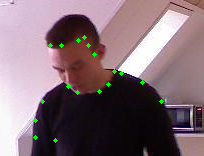
\includegraphics[width=\columnwidth]{RGBregistered.png}%
	\caption{}%
	\label{}%
\end{subfigure}
\begin{subfigure}[b]{0.48\columnwidth}
	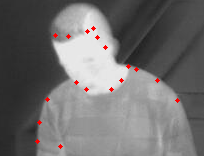
\includegraphics[width=\columnwidth]{Thermalregistered.png}%
	\caption{}%
	\label{}%
\end{subfigure}
\caption{Example of $\text{RGB (a)} \Rightarrow \text{thermal (b)}$ registration.}
\label{fig:registeredImagery}
\end{figure}

\section{Trimodal human body segmentation}
\label{sec:trimodalhumanbodysegmentation}

Let us write $\mathbf{F}_i = \{\mathbf{C}_i, \mathbf{D}_i, \mathbf{T}_i\}$ for a determined tri-modal frame, and $\mathbf{p}$ a pixel at an arbitrary location $(x,y)$ in an image.

\subsection{Extraction of masks and regions of interest} 
\label{ssec:bsbb}

% introductory sentence or paragraph missed

\subsubsection{Background subtraction}\label{sect:bs}
The first step of our baseline is to attempt to reduce the search space. A static videocamera with fixed orientation observing an indoor scene is a common practice which enables to detect and isolate new objects entering the scene assuming that the images of the scene without new objects, known as background, exhibit some regular behavior that can be described by a statistical model. Thus, in order to perform background subtraction one has first to learn a model of the background. Once learned, this model is compared against the new incoming images and parts that do not fit are considered foreground. A widely used approach for background modeling in this context is Mixture of Gaussians MOG  \cite{bouwmans2008background}, which assigns a GMM per pixel with a fixed number of components. Sometimes background presents periodically moving parts such as noise or sudden and gradual illumination changes. Such problems are often tackled with adaptive algorithms that keep learning the pixel's intensity distribution after the learning stage with a decreased learning rate. However, this also causes that intruding objects that stand still for a period of time vanish, so in our case a non-adaptive approach is more convenient.

Although this background subtraction technique performs fairly well, it has to deal with the intrinsic problems of the different image modalities. For instance, color-based algorithms may fail due to shadows, similarities in color between foreground and background, highlighted regions, and sudden lighting changes. Thermal imagery may also have this kind of problems, plus the inconvenience of temperature changes in objects. A halo effect is also observed around warm items. Regarding to depth-based approaches, they may produce misdetections due to the presence of foreground objects with similar depth to the background. However, they are more robust to lighting artifacts and shadows. Depth data is quite noisy and many pixels in the image may have no depth due to multiple reflections, transparent objects, or scattering in certain surfaces such as human tissue and hair. Furthermore, a halo effect around humans or objects is usually perceived due to parallax issues. A comparison is shown in Fig. \ref{fig:bscomparison}, where the actual foreground objects are the human and the objects on the table. As we can observe, RGB fails at extracting the human legs due to the similarities in color with the chair at the back. The thermal cue segments the human body more accurately, but includes some undesired reflections and the jar and mugs with a surrounding halo. The pipe tube is also extracted as foreground due to temperature changes along time. Despite its drawbacks, depth-based background subtraction is the one that seems to give the most accurate result. 

Therefore, the binary foreground masks of our proposed baseline are computed applying background subtraction to the depth modality previously registered to the RGB one, thus allowing us to use the same masks for both modalities.  Let us consider the depth value of a pixel at frame $i$ as $\mathbf{d}_i$. The background model $p(\mathbf{d}_i|BG)$ --where $BG$ represents the background -- is estimated from a training set of depth images represented by $\mathcal{D}$ using the $T$ first frames of a sequence such that $\mathcal{D} = \{\mathbf{d}_1, \ldots, \mathbf{d}_T\}$. This way, the estimated model is denoted by $\hat{p}(\mathbf{d}_i| \mathcal{D}, BG)\}$, modeled as a mixture of gaussians. In particular, we use the available implementation in OpenCV of the method presented in \cite{zivkovic2004improved}, which uses an on-line clustering algorithm that constantly adapts the number of components of the mixture for each pixel during the learning stage. GMMs are further explained in section \ref{section:gmm}.

Once the binary foreground masks are obtained, a 2-D connected component analysis is performed using basic mathematical morphological operators and setting a minimum value for each connected component area (except in left and rightmost sides of the image which may be caused by a new incoming item) to clean the noisy output mask. On another front, foreground masks for the thermal modality are computed using the provided registration algorithm with the depth/color foreground masks as input. From now on, we will use $FG = \{FG^\mathrm{color}, FG^\mathrm{depth}, FG^\mathrm{thermal}\}$ to refer to them. 
 
 \begin{figure}[!h]
{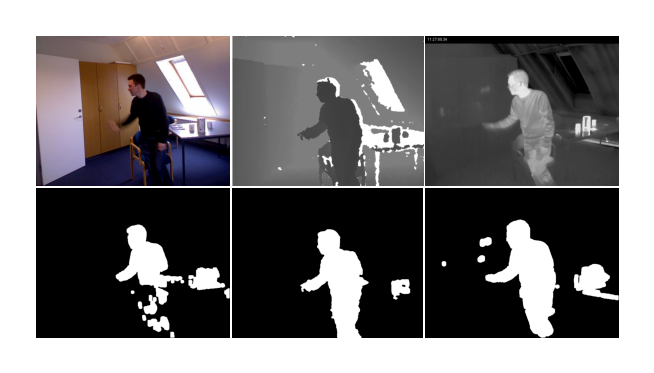
\includegraphics[width=\linewidth]{bs.eps}}
\caption{Background subtraction for different visual
modalities of the same scene (RGB, depth and thermal respectively).
\label{fig:bscomparison}}
\end{figure}

\subsubsection{Bounding box generation from regions of interest}
\label{sssec:bbgen}
To further process the information of each connected component of the previously extracted depth-based foreground masks, rectangular bounding boxes are to be generated encapsulating such components individually over time, whose function is to denote the regions of interest of a foreground mask. This way, we define the set of bounding boxes of the $i$-th frame generated from the depth-based masks as $B^\mathrm{depth}_i = \{b_{ij}\text{ }|\text{ }\forall j = \{1, \ldots, n\} \}$, being $b_{ij}$ the $j$-th bounding box and $n$ the number of bounding boxes generated in that frame, which is equal to the number of connected components. Similarly, bounding boxes generated from the resulting thermal masks are denoted by $B^\mathrm{thermal}_i$. Since color and depth modalities share the same foreground masks, $B^\mathrm{depth}_i = B^\mathrm{color}_i$, having also the same number of bounding boxes, condition that $B^\mathrm{thermal}_i$ does not currently fulfill. At the end, each frame will have to contain the same number of bounding boxes in each one of the modalities, which in turn have to correspond to the same regions of interest among them in order to allow a proper comparison. This issue will be tackled in section \ref{sssec:cpcode}.

A region of interest $r \in R$ should contain a separated person or object. However, different subjects or objects may overlap in space, resulting in a bigger component containing more than one item, for this reason each component has to be analyzed to find the correct bounding boxes that surround each region of interest. One of the advantages of the depth cue is that we can use the depth value in each range pixel to know whether an item is farther or not than other. We can assume that a given connected component belongs to just one item if its disparity distribution has a low standard deviation, that is, there is no rapid change in disparity. For those that have a greater standard deviation, Otsu's method \cite{otsu1975threshold} can be used to split the blob by automatically finding a threshold assuming a bimodal distribution. It calculates the optimal threshold separating the two classes such that their intra-class variance is minimal. We will define $\pi$ as the function that applies this method to a set of bounding boxes.

For such purpose, we define $\mathbf{c}$ as a vector containing the depth range values that correspond to a given connected component, with mean $\mu_{c}$ and standard deviation $\sigma_{c}$, and $\sigma_\mathrm{otsu}$ as a parameter that defines the maximum $\sigma_{c}$ allowed to not apply $\pi$. Note that erroneous white or black pixels do not have to be taken into account in $\mathbf{c}$ when finding the Otsu's threshold because they would change the disparity distribution, thus leading to incorrect divisions. Hence, if $\sigma_{c} > \sigma_\mathrm{otsu}$,  $\pi$ is applied. However, the assumption of bimodal distribution may not hold, so to take into account the possibility of more than two overlapping items the process is applied recursively to the divided regions in order to extract all of them. 

Once the different items are found, the regions belonging to them are labeled using a different id per item. Besides, they are again surrounded by new bounding boxes denoted by: 

\begin{gather}
O^\mathrm{depth}_i = \big\{ o_{im} | \forall m = \{1, \ldots, M_n \}_j \big\}
\end{gather}
where $\{o_{im}\}_j$ is the set of new $M_n$ bounding boxes generated by the bounding box $b_{ij}$.

\subsubsection{Bounding box transformation and correspondence to other modalities} 
\label{sssec:cpcode}
%in Section \ref{sect:bs} 
As stated previously, depth and color cues use the same foreground masks, so we can take advantage of the same bounding boxes for both modalities. However, since the thermal cue uses a transformation of these masks by applying the registration algorithm frame by frame, new bounding boxes with different coordinates are computed for that modality, which must correspond to the same regions of interest of the depth and color cues. In case of overlapping items, it would suffice by finding the registered labeled connected components to generate the new bounding boxes. Unfortunately, the algorithm cannot register connected components up to a pixel level, meaning that those that have more than one id in depth or color masks would have just one id in thermal ones, thus being surrounded by just one big bounding box. The problem here is twofold: (1) find the correspondence between $B^\mathrm{depth}_i$ and $B^\mathrm{thermal}_i$ such that a bounding box of $B^\mathrm{depth}_i$ and the matched one of $B^\mathrm{thermal}_i$ contain the same region of interest $r$; and (2), if a bounding box from $B^\mathrm{depth}_i$ was modified after $\pi$, compute the corresponding sub bounding boxes that belong to the matching bounding box in $B^\mathrm{thermal}_i$.   

The correspondence task (1) is achieved using an iterative algorithm that, taking into account the deviation among depth/color and thermal modalities, searches for the bounding boxes that match the best, both in terms of bounding box coordinates and area similarity. The correspondence function is denoted as:
\begin{gather}
b^\mathrm{thermal}_{iq} =  \beta(b^\mathrm{depth}_{ij})
\end{gather}
 
Bounding boxes of both sets are ordered beforehand in a row-major order using the top-left corner of the bounding box as a reference, thereby easing the search task. Bounding boxes which appear in thermal but do not have a correspondence in depth are omitted, whereas those in the depth modality that do not have a correspondence either are copied as they are, that is, with the same coordinates, following one of the main aforesaid constraints which states that the number of bounding boxes must be the same among modalities.

 Once we have found the correspondence between both sets, we can use the information stored in $O^\mathrm{depth}_i$ in order to address the task of bounding box splitting (2). Let us define $h_{b^\mathrm{thermal}_{iq}}$ and $v_{b^\mathrm{thermal}_{iq}}$ as the height and width of a thermal bounding box respectively, and similarly for depth bounding boxes $h_{b^\mathrm{depth}_{ij}}$ and $v_{b^\mathrm{depth}_{ij}}$, such that $b^\mathrm{thermal}_{iq} =  \beta(b^\mathrm{depth}_{ij})$. Given the deviation among modalities, we assume that the dimensions of two matched bounding boxes are proportional.  Therefore, $h_{b^\mathrm{thermal}_{iq}} \propto h_{b^\mathrm{depth}_{ij}}$ and  $v_{b^\mathrm{thermal}_{iq}} \propto v_{b^\mathrm{depth}_{ij}}$. Thus, the ratio between both bounding boxes is:

\begin{gather}
k_\text{h} = \frac{h_{b^\mathrm{depth}_{ij}}}{h_{b^\mathrm{thermal}_{iq}}}\\[2ex]
k_\text{v} = \frac{v_{b^\mathrm{depth}_{ij}}}{v_{b^\mathrm{thermal}_{iq}}}
\end{gather}

Such ratio can be utilize to create a new bounding box $o^\mathrm{thermal}_{ik} \in O^\mathrm{thermal}_i $ in such a vay that its dimensions are:

\begin{gather}
h_{o^\mathrm{thermal}_{ik}} =  k_\text{h} h_{o^\mathrm{depth}_{ij}}  \\[2ex]
v_{o^\mathrm{thermal}_{ik}} =  k_\text{v} v_{o^\mathrm{depth}_{ij}} 
\end{gather}

The expansion or shrinking of $o^\mathrm{thermal}_{ik}$ is produced taking as reference the center of $o^\mathrm{depth}_{ij}$, considering the boundaries of $b^\mathrm{thermal}_{iq}$ as the growth limit, meaning that if the new bounding box has to expand vertically but it reaches the bottom of $b^\mathrm{thermal}_{iq}$, it will stop expanding downwards but will continue doing so upwards, and similarly for left and right sides, until reaching the desired measures if possible. 

As a result, we obtain the final set of bounding boxes $O^\mathrm{thermal} \equiv O^\mathrm{depth} = O^\mathrm{color}$, which although not having the same coordinates denote the same regions of interest $R$. Henceforth, we will simply use $R$ to refer to such regions.

\subsection{Grid partitioning}
\label{ssec:gridpartitioning}

Given the precision got in the registration, particularly because of the depth-to-thermal transformation, we are not able to make a pixel-to-pixel correspondence among all the modalities. Instead, the association is made among greater information units: grid cells. 

Each region of interest $r \in R$ associated to either a segmented subject or object is partitioned in a grid of cells. We write $G_{rij}$ to refer to the position $(i,j)$ in the $r$-th region, such that $i \in \{ 1,...,v_\mathrm{grid} \}$ and $j \in \{ 1,...,h_\mathrm{grid} \}$. Regarding to the whole set of $(i,j)$-cells $\{G_{rij}\}_{\forall r \in R}$, it is denoted by $G_{ij}$.

In turn, a grid cell $G_{rij}$ consists in a set of image subregions $\{\mathbf{G}_{rij}^c\}_{\forall{c} \in \mathcal{C}}$, provided by the set of visual cues $\mathcal{C} = \{\mathrm{color}, \mathrm{depth}, \mathrm{thermal}\}$. Accordingly, $\{\mathbf{G}_{rij}^c\}_{\forall r \in R}$, the set of $(i,j)$-cells in the modality $c$, is indicated by $G_{ij}^c$.

The grid cell is the unit of information processed in the different modalities' description and classification procedures. The next section provides the details about the feature extraction computed from different visual cues at cell level.

\subsection{Feature extraction}
\label{ssec:feature extraction}

Each modality involves its own specific descriptors. In the case of the color modality two kind of descriptors are extracted for each cell, Histogram of Oriented Gradients (HOG) and Histogram of Oriented Optical Flows (HOOF), whereas in the depth and thermal modality the Histogram of Oriented Normals (HON) and Histogram of Intensities and Oriented Gradients (HIOG) are respectively computed. Eventually, from this feature extraction process, a set of descriptions is obtained $D_{ij} = \{\mathbf{D}_{ij}^d\}_{\forall d \in \mathcal{D}}$ for each grid position $(i,j)$, being $\mathcal{D}$ the set of considered descriptors $\{\mathrm{HOG}, \mathrm{HOOF}, \mathrm{HON}, \mathrm{HIOG}\}$.

The color modality is also used to compute a sequence of probability-like maps at pixel-level (SM). Such descriptor is also included in this section but for the moment is not included in the set of descriptions $\mathcal{D}$, owing to the fact that its intrinsic characteristics differ from the others and will be treated in a distinct fashion.

\subsubsection{Color}
\label{sssec:color}

The color cue is nowadays the most popular imagery modality and has been extensively used to extract a range of different feature descriptions. It is usually represented by the RGB color space, which expresses the color as a triplet $(\text{red}, \text{green}, \text{blue})$, but other models are also available. Notwithstanding its simplicity and properties, it suffer from some drawbacks such as illumination changes, shadows, camouflage, among others, which may inconvenience some tasks.

\begin{figure}
        %add desired spacing between images, e. g. ~, \quad, \qquad etc.
         %(or a blank line to force the subfigure onto a new line)
        \begin{subfigure}[b]{0.515\textwidth}
                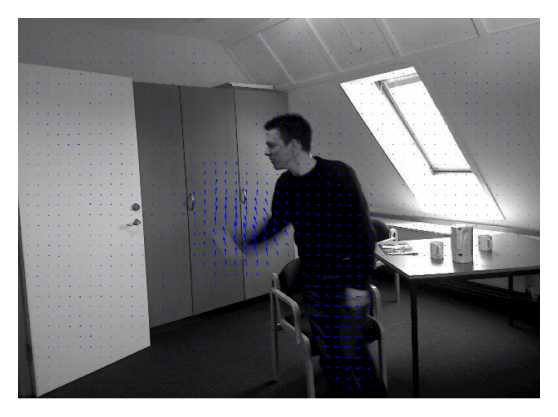
\includegraphics[width=\textwidth]{opticalflow_final.eps}
                \caption{Optical flow}
                \label{fig:opticalflow}
        \end{subfigure}
        \begin{subfigure}[b]{0.5\textwidth}
                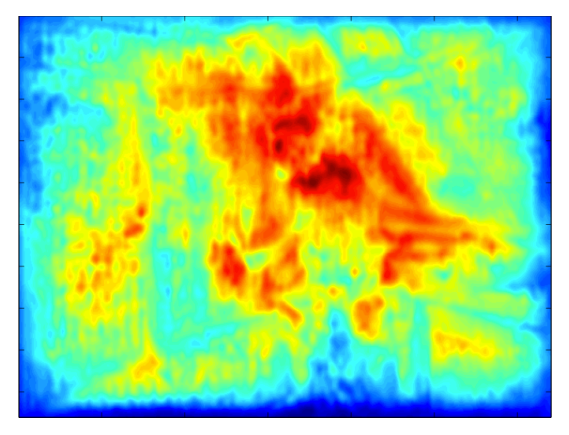
\includegraphics[width=\textwidth]{ramanan_final}
                \caption{Ramanan score map}
                \label{fig:ramanan}
        \end{subfigure}
        \begin{subfigure}[b]{0.5\textwidth}
                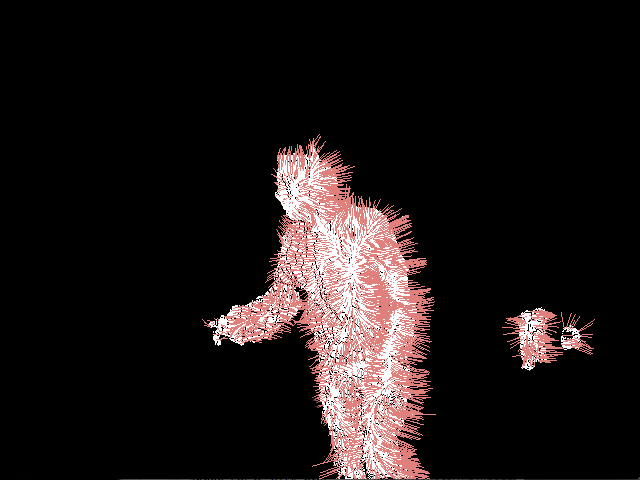
\includegraphics[width=\textwidth]{normals.png}
                \caption{Depth normals}
                \label{fig:normals}
        \end{subfigure}
        \begin{subfigure}[b]{0.5\textwidth}
                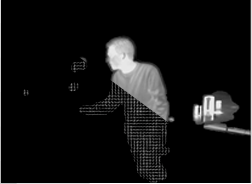
\includegraphics[width=\textwidth]{hihog.png}
                \caption{Thermal intensities and oriented gradients}
                \label{fig:thermals}
        \end{subfigure}	
        \caption{Example of descriptors from RGB modality: (A) represents the motion vectors using a forward scheme, that is, the optical flow orientation gives insight into where the person is moving to in the next frame; (B) score maps representing the hypothesis of a pixel belonging to a person; (C) the computed surface normal vectors; (D) the intensity and the thermal gradients orientations. }\label{fig:descriptors}
\end{figure}

\paragraph{Histogram of oriented gradients (HOG)}
For RGB cue, a simple implementation of HOG \cite{dalal2005histograms} is to be computed for each grid cell, known as detection window in the HOG context. Each window is resized to a $h_\mathrm{w}^\mathrm{HOG} \times v_\mathrm{w}^\mathrm{HOG}$ pixel area and divided in rectangular blocks of $h_\mathrm{b}^\mathrm{HOG} \times v_\mathrm{b}^\mathrm{HOG}$ pixels, which are in turn divided into rectangular local spatial regions called cells of size $h_\mathrm{c}^\mathrm{HOG} \times v_\mathrm{c}^\mathrm{HOG}$ pixels, thus having 4 cells per block and 8 blocks per window. We use RGB color space with no gamma correction. In order to compute the gradients, two kernels in the x and y directions with no smoothing are used for each channel so as to find and take the channel with the greatest gradient magnitude for each pixel. The gradient at point $\mathbf{p}$ of detection window is:

\begin{gather}
\mathcal{G}_\mathbf{p}^x = \mbox{[-1 0 1]} \ast \mathbf{C}_\mathbf{p} \label{eq:gx} \\[2ex]
\mathcal{G}_\mathbf{p}^y = \mbox{[-1 0 1]}^\mathrm{T} \ast \mathbf{C}_\mathbf{p} \label{eq:gy}
\end{gather}

The gradient magnitude $\mathbf{M}$ and orientation $\mathbf{\Theta}$ of the gradient at point $\mathbf{p}$ are:

\begin{gather}
\mathbf{M}_{\mathbf{p}} = \sqrt{(\mathcal{G}_{\mathbf{p}}^{\mathrm{x}})^2 + (\mathcal{G}_{\mathbf{p}}^{\mathrm{y}})^2} \label{eq:magnitude}\\[2ex]
\mathbf{\Theta}_{\mathbf{p}} = \tan^{-1} \Big(\frac{\mathcal{G}_{\mathbf{p}}^{\mathrm{y}}}{\mathcal{G}_{\mathbf{p}}^{\mathrm{x}}}\Big) \label{eq:orientation}
\end{gather}

Gradient orientation is also computed for each pixel in the dominant channel and assigned into a $\kappa$-bin histogram over each cell using unsigned gradients such that bins are evenly spaced over $0^\circ$ and $180^\circ$. As stated in \cite{dalal2005histograms}, signed contrast is uninformative for humans due to the wide range of clothing and background colors. For each gradient vector, its contribution to the histogram is given by the vector magnitude, that is, stronger magnitudes have a bigger impact on the histogram. Owing to local variations in illumination and foreground-background contrast gradient strengths vary over a wide range so cells are grouped into larger, spatially connected blocks. Hence, the information of each cell is concatenated. Then, the gradient strengths are locally normalized applying the L2-norm over each block. Block overlap is not applied in this case so as to lower the final descriptor dimensions. 

\paragraph{Histogram of oriented optical flow (HOOF)} 
Since we are working with video sequences, the color cue also allows us to obtain motion information by computing dense optical flow and describing the distribution of the resultant vectors, known as histogram of oriented optical flow \cite{dalal2006human}. The optical-flow vectors of the whole image are computed using the luminance information of the image with the Gunnar Farneb\"{a}ck's algorithm \cite{farneback2003two} available in OpenCV\footnote{\url{http://code.opencv.org.}} \cite{bradski2008learning}, which is based on modeling the neighborhoods of each pixel of two consecutive frames by quadratic polynomials. It represents the image signal in the neighborhood of each pixel by a 3-D surface and finds where the surface has moved in the next frame. As a result, a set of 2-D vectors denoting the movement of each pixel for the horizontal $\mathbf{u}$ and vertical $\mathbf{v}$ directions in the compared frames is found. It allows a wide range of parameterizations, which will be specified in section \ref{ch:evaluation}.

 The resulting motion vectors, whose example is shown in Fig. \ref{fig:opticalflow}, are masked and quantized to produce weighted votes for local motion based on their magnitude which are locally accumulated into a $\nu$-bin histogram over each grid cell according to the signed ($0^\circ$ - $360^\circ$) vector orientations. In contrast to HOG, HOOF uses signed optical flow since the orientation provides more discriminative power. Magnitude and orientation of a motion vector at pixel $\mathbf{p}$ are calculated as in Eq. \ref{eq:magnitude} and Eq. \ref{eq:orientation} respectively.

\subsubsection{Depth}
\label{sssec:depth}

The grid cells in the depth modality $\mathbf{G}_{ij}^\mathrm{depth}$ are depth dense maps represented as planar images of pixels (in projective coordinates) that take depth values in millimeters. From the depth representation in projective coordinates it is possible to obtain the "real world" ones by using the intrinsic parameters of the depth sensor. This conversion generates 3-D point cloud structures $\mathcal{P}_{ij}$ in which the distances among points are actual distances -- those that can be measured in the real world. Finally, in each point cloud $\mathcal{P}_{rij} \in \mathcal{P}_{ij}$ the surface normals are computed and their angles' distribution summarized in a $\delta$-bin histogram, eventually describing the cell from the depth modality point of view.

\paragraph{Histogram of oriented depth normals (HON)} 
In order to describe an arbitrary point cloud $\mathcal{P}$ the surface normals vectors have to be computed first. A surface normal of a 3-D point is a perpendicular vector to a 3-D plane which is tangent to the surface in that point. Thus, the normal 3-D vector at a given point $\mathbf{p} = (p_x, p_y, p_z) \in \mathcal{P}$ can be seen as the problem of determining the normal of a 3-D plane tangent to $\mathbf{p}$. A plane is represented by the origin point $\mathbf{q}$ and the normal vector $\mathbf{n}$. From the neighboring points $\mathcal{K}$ of $\mathbf{p} \in \mathcal{P}$, we first set $\mathbf{q}$ to be the average of those points:

\begin{gather}
	\mathbf{q} \equiv \bar{\mathbf{p}} = \frac{1}{|\mathcal{K}|} \sum_{\mathbf{p} \in \mathcal{P}^{\mathcal{K}}} \mathbf{p}
\end{gather}
 
Then, the solution of $\mathbf{n}$ can be approximated using the covariance matrix $C \in \mathbb{R}^{3 \times 3}$ of the points in $\mathcal{P}_\mathbf{p}^{\mathcal{K}}$. The covariance matrix $C$ is computed as follows: 

\begin{gather}
	C = \frac{1}{|\mathcal{K}|} \sum_{i=1}^{|\mathcal{K}|} (\mathbf{p}_i - \bar{\mathbf{p}}) (\mathbf{p}_i - \bar{\mathbf{p}})^{\mathrm{T}}
\end{gather}
being $C$ a symmetric positive semi-definite matrix. Solving the next equation by means of eigenvalue decomposition:

\begin{gather}
	C \mathbf{u}_j = \lambda_j \mathbf{u}_j, \; j \in \{0,1,2\}
\end{gather}
where $\lambda_j \in \mathbb{R}$ and $\mathbf{u}_j \in \mathbb{R}^3$ represent the $j$-th eigenvalue and eigenvector of $C$ respectively, a solution for $\mathbf{n}$ is found to be the eigenvector $\mathbf{u}_j$ with the associated smaller $\lambda_j$. Formally,

% fix argmin
\begin{gather}
	\mathbf{n} = \mathbf{u}_z, \;\; \mathrm{where}  z = \argmin_{j}{\lambda_j}, j \in \{0,1,2\}
\end{gather}

The sign of $\mathbf{n}$ can be either positive or negative, and it can not be disambiguated from the calculations. We adopt the convention of re-orienting consistently all the computed normal vectors towards the depth sensor's viewpoint $\mathbf{z}$. The computed normal vectors over a human body region is shown in Figure~\ref{fig:normals}. Points are illustrated in white, whereas normal vectors are red lines (instead of arrows for the sake of the visual comprehension). The next step is to build the histogram describing the distribution of the normal vectors' orientations.

A 3-D normal vector got from the previous calculations is expressed in cartesian coordinates $(n_x, n_y, n_z)$. Nonetheless, a normal vector can be also expressed in spherical coordinates using three parameters: the radius $s$, the inclination $\theta$, and the azimuth $\varphi$. In our case, $s$ is a constant value, so this parameter can be omitted. Regarding $\theta$ and $\varphi$, the cartesian to spherical coordinates transformation is calculated as:

% fix atan
\begin{gather}	
	\theta  = \atan{\left( \frac{n_z}{n_y} \right)},
	\varphi = \acos{\frac{ \sqrt{(n_y^2 + n_z^2)} }{n_x}}
\end{gather}

Therefore, a 3-D normal vector can be characterized by a pair ($\theta$, $\varphi$) and the depth description of a cell consists of a pair of concatenated $\delta_\theta$-bin and $\delta_\varphi$-bin histograms, describing the two angular distributions of the body surface normals within the cell. Moreover, each of the two histograms is normalized before the concatenation, dividing by the number of elements, to end up with a relative angles frequency count.

\subsubsection{Thermal}
\label{sssec:thermal}

The thermal cue is a very informative feature for the task of people detection/segmentation. A pixel part of a human region gives off heat and hence a relatively large value in terms of thermal intensity.

\paragraph{Histogram of thermal intensities and oriented gradients (HIOG)} 
The descriptor got from a cell in the thermal cue $\mathbf{G}_{rij}^{\mathrm{thermal}}$ is the concatenation of two histograms. The first one is an histogram summarizing the thermal intensities, which range in the interval $[0, 255]$. The intensities are the ones in the masked region of the cell, i.e. not taking into account the background pixels. Instead, the second histogram is summarizing the orientations of thermal gradients. These gradients are computed convolving a first derivative kernel in both directions (as in Eq.~\ref{eq:gx}-\ref{eq:gy}). Then, their orientation is calculated and binned in the histogram weighted by their magnitude. Finally, the two histograms are normalized dividing by the sum of the accumulations in the bins and concatenated. We used $\tau_{\mathrm{i}}$ bins for the intensities part and $\tau_{\mathrm{g}}$ bins for the gradients' orientations.

\subsection{Cell classification}
Since we are intended to segment human body regions, we need to distinguish those from the other foreground regions segmented by the background subtraction algorithm. These other foreground regions, apart from subjects, are the objects -- they could be other living beings, e.g. cats or dogs, though these are not considered in this work.

From the previous step, each grid cell has been described using the different descriptors $\mathcal{D}$. For the purpose of classification, we train several Gaussian Mixture Models for each grid position $(i,j)$, kind of description $d \in \mathcal{D}$, and foreground class either subject or orbject. Concretely, the set of GMMs modeled from the set of grid cells positioned in $(i,j)$ is $\mathcal{M}_{ij} = \{\mathcal{M}_{ij}^{d,\mathrm{sub}},\mathcal{M}_{ij}^{d,\mathrm{obj}}\}_{\forall d \in \mathcal{D}}$. In Fig.~\ref{fig:baseline}, the different steps of the baseline up to this point are illustrated.

\begin{figure}[ht!]
	\centering
	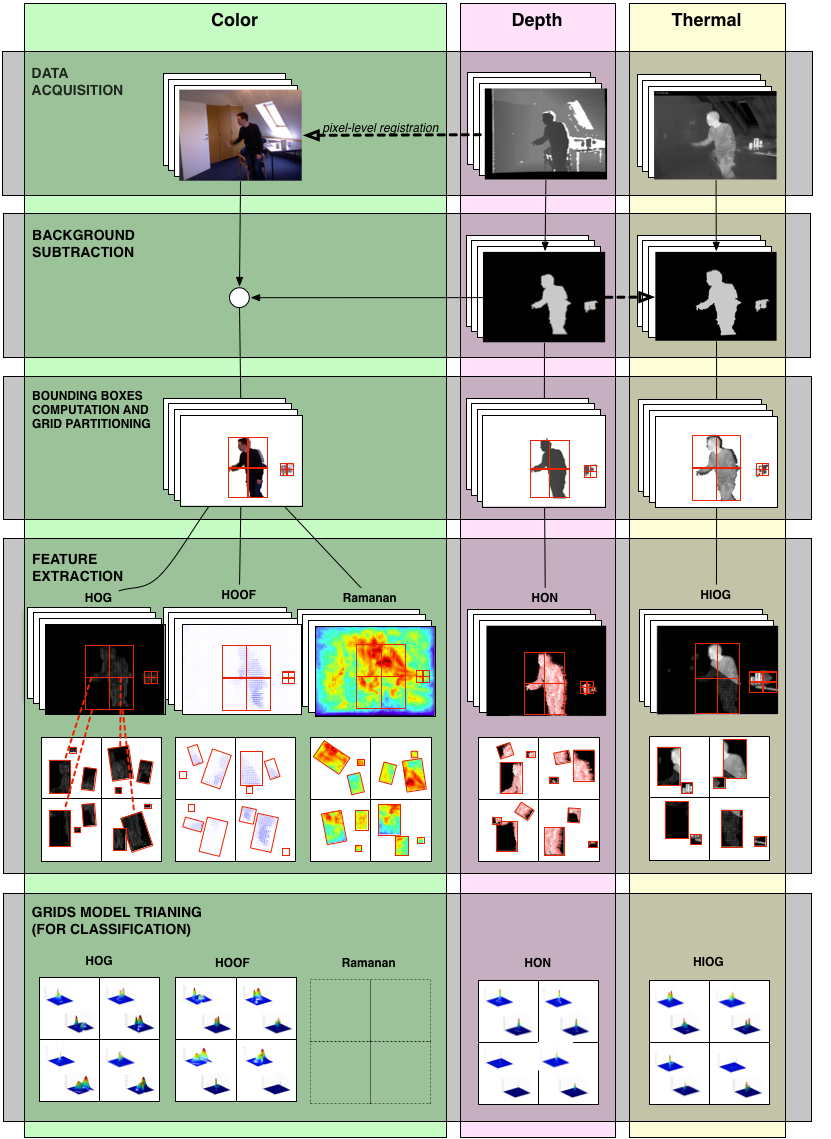
\includegraphics[width=\linewidth]{pictures/diagram.png}
	\caption{The main steps of the proposed baseline method, before reaching the fusion step.}
	\label{fig:baseline}
\end{figure}

Then, in testing time, an unseen cell can be predicted to be a subject or an object depending on the likelihood got in the probability density function (PDF) of the different mixtures. We will denote the likelihood values got from the GMMs $\mathcal{M}_{ij}^{d,\mathrm{sub}}$ and $\mathcal{M}_{ij}^{d,\mathrm{obj}}$ by $\mathcal{L}_{ij}^{d,\mathrm{sub}}$ and $\mathcal{L}_{ij}^{d,\mathrm{obj}}$ respectively. The final classification of a $G_{rij}$ is performed by combining somehow and comparing $\{\mathcal{L}_{rij}^{d,\mathrm{sub}}\}_{\forall d \in \mathcal{D}}$ and $\{\mathcal{L}_{rij}^{d,\mathrm{obj}}\}_{\forall d \in \mathcal{D}}$. How to intelligently combine the previous classification results is explained in Section~\ref{ssec:fusion}.

\subsubsection{Gaussian Mixture Models} \label{section:gmm}

Gaussian Mixture Models (GMMs) is an unsupervised learning method for fitting multiple Gaussians to a set of multi-dimensional data points\footnote{This technique uses properties of gaussians, thus its generalization to fit other functions is not straightforward.}. It is often used as a probabilistic clustering and an alternative to the k-means algorithm. As in the case of k-means, the number of components $K$ (or gaussians) in the mixture is a parameter that needs to be specified to the algorithm. The GMMs are trained using the very general Expectation-Maximization algorithm~\cite{moon1996expectation}. The goal is to end up maximizing the overall likelihood $\mathcal{L}$ of the model:

\begin{gather}
	\mathcal{L} = \prod_{\mathbf{x} \in \mathbf{X}}^{N} p(\mathbf{x})
\end{gather}
where $\mathbf{x}$ is a multi-dimensional data point (in this case representing the descriptor of an arbitrary grid cell $\mathbf{G}_{rij}^{d}$) and $p(\mathbf{x})$ is the probability of $\mathbf{x}$ being drawn from the model. This probability is the value assigned by the mixture PDF to that point, which is in fact a linear combination of $K$ gaussian PDFs:

\begin{gather}
	p(\mathbf{x}) = \prod_{k=1}^{K} p(\mathbf{x}|k) P(k)
\end{gather}
being $p(\mathbf{x}|k)$ the value assigned by the $k$-th gaussian PDF to $\mathbf{x}$ (the height of the PDF function at that point), whereas $P(k)$ is the importance, or weight, of the $k$-th component in the mixture. In fact, since the model is a mixture of gaussians, $p(\mathbf{x})$ can be expressed as the mixture of parametrized gaussian functions:

\begin{gather}
	p(\mathbf{x}) = \prod_{k=1}^{K} \mathcal{N}(\mathbf{x}|\boldsymbol{\mu}_{k}, \mathbf{\Sigma}_{k}) P(k), \\
	\mathcal{N}(\mathbf{x}|\boldsymbol{\mu},\mathbf{\Sigma}) = \frac{1}{2\pi^{\rho/2}|\mathbf{\Sigma}|^{1/2}} \exp^{-\frac{1}{2} (\mathbf{x}-\boldsymbol{\mu})^\mathrm{T} \mathbf{\Sigma}^{-1} (\mathbf{x}-\boldsymbol{\mu}) }
\end{gather}

In order to be able to predict at some point new given examples, a training procedure is needed to model the parameters of the mixture, i.e. the means $\boldsymbol{\mu} = \{ \mathbf{\boldsymbol{\mu}}_1, ..., \boldsymbol{\mu}_K \}$ and covariances matrices $\mathbf{\Sigma} = \{ \mathbf{\Sigma}_1, ..., \mathbf{\Sigma}_K \}$. This is done by the two-step procedure called Expectaction-Maximization.

\subsubsection{Expectation-Maximization: modeling a GMM}

Let be $\mathbf{X}$ the set of $\rho$-dimensional points and have initialized the parameters for the $K$ components $\boldsymbol{\mu}$ and $\mathbf{\Sigma}$ and the contribution of the components $\{P(k_1), ..., P(k_K)\}$. The first step to perform is the expectation calculation, or \emph{E-Step}, that consists on computing the $K$ posteriors for all the points $\mathbf{x} \in \mathbf{X}$. The posterior $P(k|\mathbf{x})$ is the probability the point $\mathbf{x}$ belongs to the component $k$, and it is exactly:

\begin{gather}
	p_{k\mathbf{x}} = P(k|\mathbf{x}) = \frac{\mathcal{N}(\mathbf{x}|\boldsymbol{\mu}_{k}, \mathbf{\Sigma}_{k}) P(k)}{p(\mathbf{x})}
\end{gather}

Next, it is the turn of the maximization step, or \emph{M-step}. In this step, it is supposed the assignments of individual points are known but not the model. The parameters of the components and their weights are re-estimated -- because of the previous calculations -- as:

\begin{gather}
	\hat{\boldsymbol{\mu}}_k = \frac{\sum_{\mathbf{x} \in \mathbf{X}} p_{k\mathbf{x}} \, \mathbf{x}}{\sum_{\mathbf{x} \in \mathbf{X}} p_{k\mathbf{x}}} \\
	~
	\hat{\mathbf{\Sigma}}_k = \frac{\sum_{\mathbf{x} \in \mathbf{X}} p_{k\mathbf{x}} \, (\mathbf{x}_i - \hat{\boldsymbol{\mu}}_k)(\mathbf{x} - \hat{\boldsymbol{\mu}}_k)^{\mathrm{T}} }{\sum_{\mathbf{x} \in \mathbf{X}} p_{k\mathbf{x}}}\\
	~
	\hat{P}(k) = \frac{1}{|\mathbf{X}|} \sum_{\mathbf{x} \in \mathbf{X}} p_{k\mathbf{x}}
\end{gather}

It can be proven that alternating E and M steps, the algorithm converges to at least a local maximum of overall likelihoods. A typical initialization is to start with $K$ randomly chosen data points as starting means, and equal covariance matrices. Nonetheless, convergence is sometimes slow, because of having many points laying in "plateaus". Another possibility, as it has been done in this work, is to use \emph{k-means} to have a better initialization because of a more robust estimate of the initial parameters, increasing the convergence speed and the chances of finding a better solution.

Moreover, though not explained, dealing with likelihoods may cause underflow problems in the computations. The approach to cope with this problem is to apply logarithms, that is dealing with log-likelihoods instead of likelihoods. Despite this changes some calculations re-formulated using the what is called "log-sum-exp" trick, the EM algorithm is still a valid approach to maximize the log-likelihood of the model given $\mathbf{X}$.

\subsection{Multi-modal fusion} 
\label{ssec:fusion}
Having different modalities and descriptions allow us to fuse them to have a more informative and richer representation of the scenario which in turn can improve the final segmentation result. Such fusion can be achieved using several approaches, which are detailed below.  
 
Before fusing the results got in the GMMs from different modalities and classes, a normalization step is required. The more simple possible strategy that normally yields good results is to perform a min-max normalization. This is done simply by subtracting the min value of a set of values and dividing by the difference between the max and the min. In our case, the normalization is done within the set of log-likelihoods $\Delta_{ij}^d = \{\mathcal{L}_{ij}^{d,\mathrm{sub}},\mathcal{L}_{ij}^{d,\mathrm{obj}}\}$ obtained subject and object GMMs using a kind of description $d \in \mathcal{D}$. Concretely, a log-likelihood $\xi \in \Delta_{ij}^d$ is min-max normalized:

\begin{gather}
	\hat{\xi} = \frac{ \xi - \min (\Delta_{ij}^d) } { \max (\Delta_{ij}^d) - \min (\Delta_{ij}^d)}
\end{gather}

The normalized log-likelihoods $\hat{\mathcal{L}}_{ij}^{d,\mathrm{sub}},\hat{\mathcal{L}}_{ij}^{d,\mathrm{obj}}$ range in the interval $[0, 1]$, which will be further used to obtain the prediction $\hat{t}_{r}^{d} = \{0, 1\}$ of a region $r$, which denotes if such region belongs to an object or a subject respectively, and the predicted set of binary masks $\hat{S}$, which defines the human body segmentation.

SM description has not been taken into account thus far owing to its uniqueness. However, it only can be combined with the other descriptions if they are represented in an equal manner. For this purpose, a set of object score maps is computed from the original subject score maps, by taking the maximum score $\text{score}_\text{max}$ of the whole set and computing the inverse, such that:

\begin{gather}
\text{score}(p)^{obj} = \text{score}_\text{max} - \text{score}(p)^{sub}
\end{gather}

Afterwards, to modify the description to a cell level, the scores are first normalized applying, again, min-max normalization. Then, the mean is computed for each cell to obtain a value per cell, as happens in the rest of the descriptions. 

For the sake of simplicity, from this point we will consider the normalized version of SM to be part of the set of descriptors $\mathcal{D}$, and the cell probability-like values to be also part of $\Delta_{ij}^d$, even though they do not represent exactly the same.

\subsubsection{Individual prediction}
The first step is to compute the individual prediction of each of the descriptions separately. 

A grid cell voting is performed using the normalized log-likelihoods of subject and object of each of them, comparing both to decide if that cell contains a person, such that

\begin{gather}
v =  \sum_{i,j} \mathbbm{1}\{\hat{\mathcal{L}}_{ij}^{d,\mathrm{sub}} >\hat{\mathcal{L}}_{ij}^{d,\mathrm{obj}}\}
\end{gather}

We also define a threshold $v_{thr}$ that refers to the minimum number of positive votes needed to assign the subject label to the given region. Such threshold is given by

\begin{gather} \label{eq:votethr}
v_{thr} = \frac{v_\mathrm{grid}h_\mathrm{grid}}{2}
\end{gather}

However, the decision of a cell can be given by a little difference between both log-likelihoods. For this reason, in order to decide whether the region belongs to a person, such differences are taken into account if an agreement is not reached by the cells. The final decision is thus described as:
%
%\begin{gather}
%\hat{t}_{r}^{d} = \mathbbm{1} \Bigg\{ \bigg\{ v > v_{thr} \bigg\} \bigvee \bigg\{v = v_{thr} \land   \mathbbm{1}\big\{ \big( \sum_{i,j} \hat{\mathcal{L}}_{ij}^{d,\mathrm{sub}} - \hat{\mathcal{L}}_{ij}^{d,\mathrm{obj}} \big) > 0 \bigg\} \Bigg\}
%\end{gather}

\begin{gather}
\hat{t}_{r}^{d} = \mathbbm{1} \bigg\{ v > v_{thr} \bigg\} \bigvee \bigg\{ \mathbbm{1}\big\{v = v_{thr}\big\} \cdot   \mathbbm{1}\big\{ \big( \sum_{i,j} \hat{\mathcal{L}}_{ij}^{d,\mathrm{sub}} - \hat{\mathcal{L}}_{ij}^{d,\mathrm{obj}} \big) > 0 \bigg\}
\end{gather}

That is, in the event of a tie, the sum of the difference in log-likelihoods among cells would decide the final label for that region. 

In order to create the predicted segmentation masks, we use the extracted foreground masks $FG$ from the background subtraction step. For each frame, regions that belong to that frame are masked to 0 if they were predicted to be a subject, and left as they are otherwise. A prediction conflict could arise if there is an overlap between the bounding boxes that denote the regions and their labels differ. In that case, the overlapped region would be masked to 0 --thereby being considered as a subject --if, as applied before, the sum of the difference between subject and object likelihoods is negative, and kept unchanged in any other way.

\subsubsection{Naive fusion approach}
A basic fusion approach is to combine the descriptors in such a way that all contribute with equal weight. We propose a cell-level fusion using the normalized subject and object log-likelihoods and modified score maps. Consequently, a voting stage is first performed among all descriptors, whose individual predictions $\hat{t}_{r}^{d}$ are the votes, such that:

\begin{gather}
v = \sum_{d \in \mathcal{D}} \hat{t}_{r}^{d}
\end{gather}
 
Note that some of the predictions may be wrong, thereby affecting negatively the voting. If the majority of the votes consider the region to be a person, meaning that there is a strong agreement between descriptions, those descriptions that consider the given region to be a subject will not be taken into account in the cell-level fusion stage. Defining the selected descriptions as $\mathcal{D}' \subset \mathcal{D}$, their combination $\bar{\mathcal{L}}_{ij}^{d,\mathrm{sub}}$ and $\bar{\mathcal{L}}_{ij}^{d,\mathrm{obj}}$ is given by:

\begin{gather}
\bar{\mathcal{L}}_{ij}^{d,\mathrm{sub}} = \sum_{d \in \mathcal{D}'} \hat{\mathcal{L}}_{ij}^{d,\mathrm{sub}}\\[2ex]
\bar{\mathcal{L}}_{ij}^{d,\mathrm{obj}} = \sum_{d \in \mathcal{D}'} \hat{\mathcal{L}}_{ij}^{d,\mathrm{obj}}  
\end{gather}
 
Once the combined log-likelihoods are obtained, the approach follows the same procedure as the individual prediction for cell-based descriptions to obtain a final prediction $\hat{t}_r$ for each region, and similarly to obtain the segmentation masks. Note that this time, since a fused result is obtained , there will only be one set of segmented masks for all the descriptions --except for the thermal description whose $FG$ masks were different owing to the non-accurate pixel-wise registration among modalities.

\subsection{Learning-based approach}
Support vector machines is a non-probabilistic supervised binary classifier that learns a model which represents the instances as points in space, mapped in such a way that instances of different classes are separated by a hyperplane in a high dimensional space. However, if the dataset is not linearly separable in that space the hyperplane will fail in classifying properly. This can be solved by mapping the dataset instances into a higher dimensional space using a kernel function, thus making easier the dataset division \cite{hearst1998support}. 

SVM is often used in the literature as a discriminative classifier for object recognition, and particularly in human detection approaches, usually yielding successful results.  We therefore propose a fusion using SVM with different types of kernel. In particular, our baseline includes linear kernel and radial basis function (RBF). Linear SVM just requires one parameter, the penalty parameter $\zeta$, which specifies a trade-off between model complexity and misclassification of training examples and can take values in the interval $[0, inf]$. Higher values of $\zeta$ causes closer fitting to the training set, which may tend to overfitting. The performance of the RBF kernel is also influenced by the $\gamma$ parameter, which controls the shape of the separating hyperplane. Higher values usually increase the number of support vectors. Weights $\mathbf{w}$ obtained from linear SVM represent the hyperplane used to separate between classes, but they can also give us an insight of the level of importance or level of influence that each feature has when classifying the instance \cite{guyon2003introduction}. The SVM models has been trained using the available implementation of the LibSVM\footnote{\url{http://www.csie.ntu.edu.tw/~cjlin/libsvm/ }} library \cite{chang2011libsvm}.

%Such parameters have influence on the model accuracy, for that reason a proper parameter selection has to be performed

Let $\mathcal{R}$ be the data set of regions and features that will be used in the SVM approach. Each region will be described by the different probabilities of subject and object of the different descriptions $\{\hat{\mathcal{L}}_{ij}^{d,\mathrm{sub}}, \hat{\mathcal{L}}_{ij}^{d,\mathrm{obj}}\}$ such that each region $r$ will be described by $2 \times |\mathcal{D}| \times v_\mathrm{grid} \times h_\mathrm{grid}$ feature values. The computed ground truth labels $t_{r}^{m} \in T$ will be used in the training stage to indicate the class of $r$. Note that some regions have an unknown label $\{-1\}$; such regions are not used for training. Region prediction will be again denoted by $\hat{t}_r$.

However, we are not taken into account the previous predictions obtained for each description individually. In order to take into account this information, which may help in the classification stage, the set of individual predictions $\hat{t}_{r}^{d}$ can be included in the data set $\mathcal{R}$, such that each region $r$ is described by $2 \times |\mathcal{D}| \times v_\mathrm{grid} \times h_\mathrm{grid} + |\mathcal{D}|$. This approach follows the Stacked Learning scheme \cite{cohen2005stacked, gatta2011multi}, which involves training a new learning algorithm combining previous predictions obtained with other learning algorithms. 

Accordingly, we use four SVM classifiers: (1) simple linear SVM, (2) simple RBF SVM, (3) stacked linear SVM, and (4) stacked RBF SVM. Segmented masks are created following, again, the aforementioned procedure.

\section{Evaluation}
\label{sec:evaluation}
The proposed method is evaluated on a data set with a total of 11537 frames, of which 5724 frames are annotated as this requires a significant amount of resources. Sample imagery of the scenes is pictured in Figure \ref{fig:samplescenes} whereas Table \ref{tab:scenes} shows the number of annotated frames and the depth range. Activity in scene 1 and 3 is using the full depth range of the Kinect sensor whereas activity in scene 2 is constrained to a depth range of $\pm 0.250$ m. Scene 1 and 2 are situated in a closed meeting room with little natural light to disturb the depth sensing, whereas scene 3 is situated in a area with wide windows and a substantial amount of sunlight.

\begin{figure}[htbp]
	\centering
		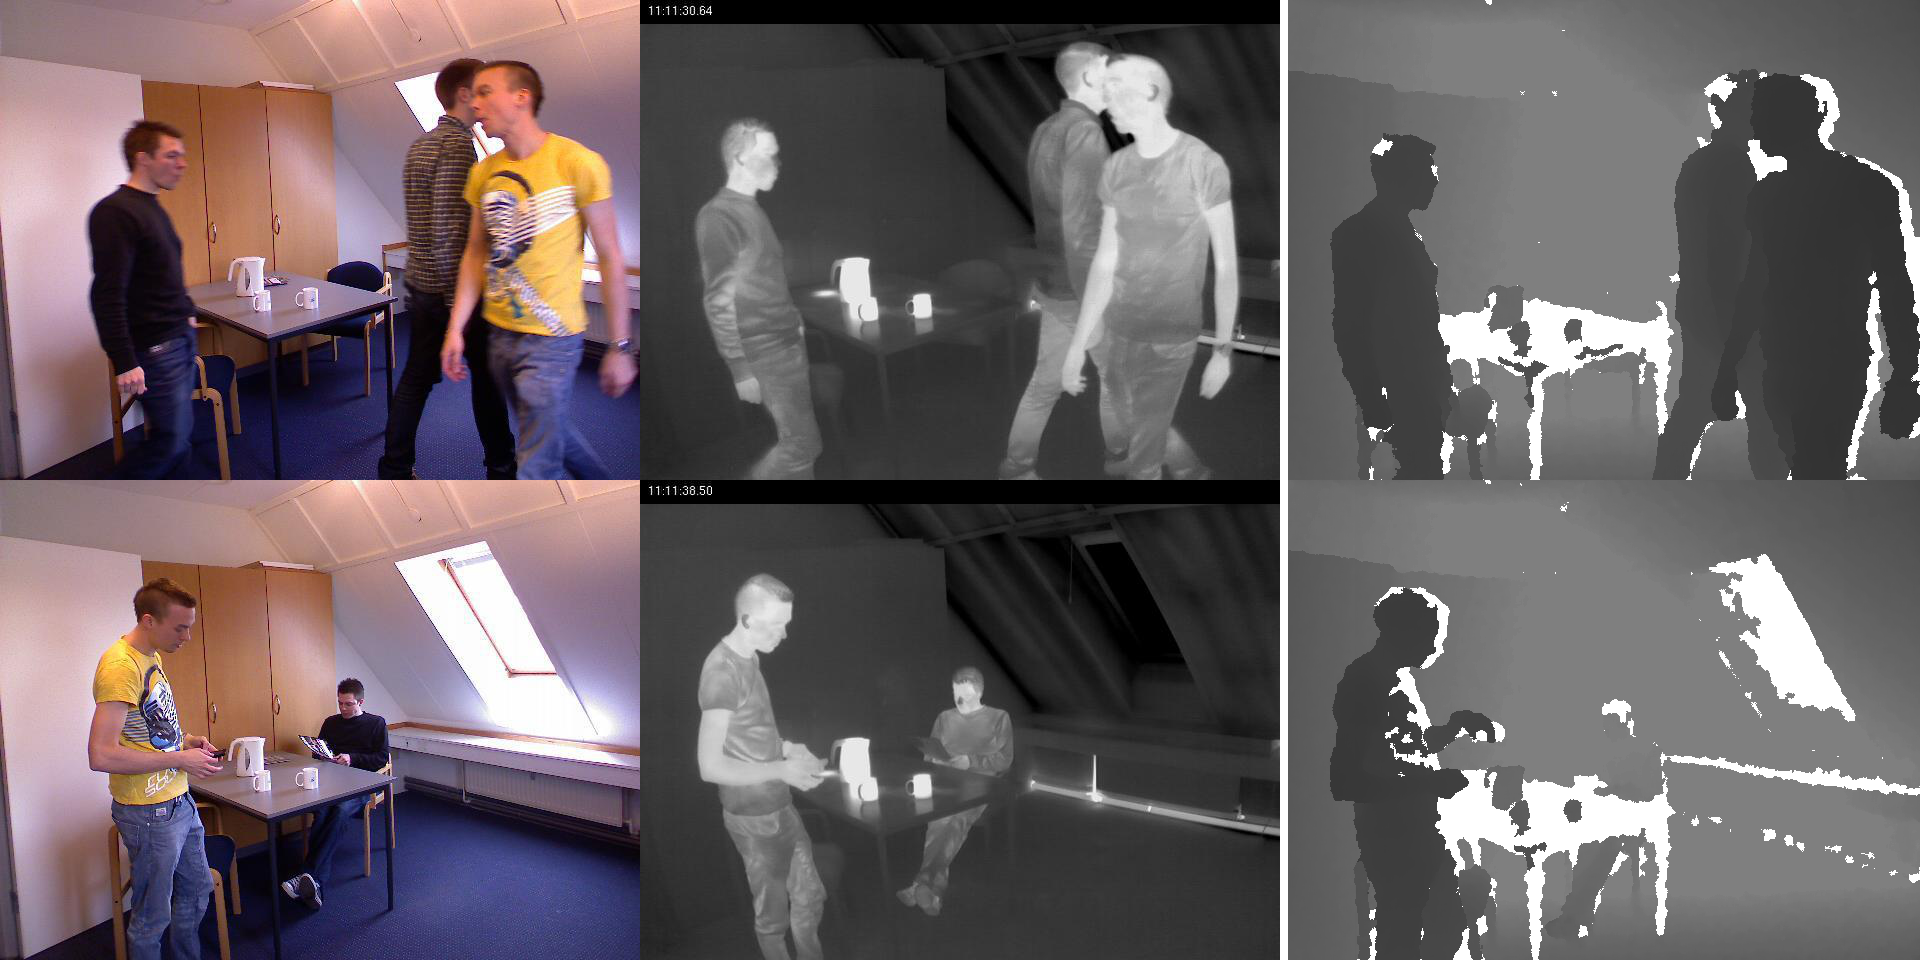
\includegraphics[width=0.48\textwidth]{Selection/1.png}
		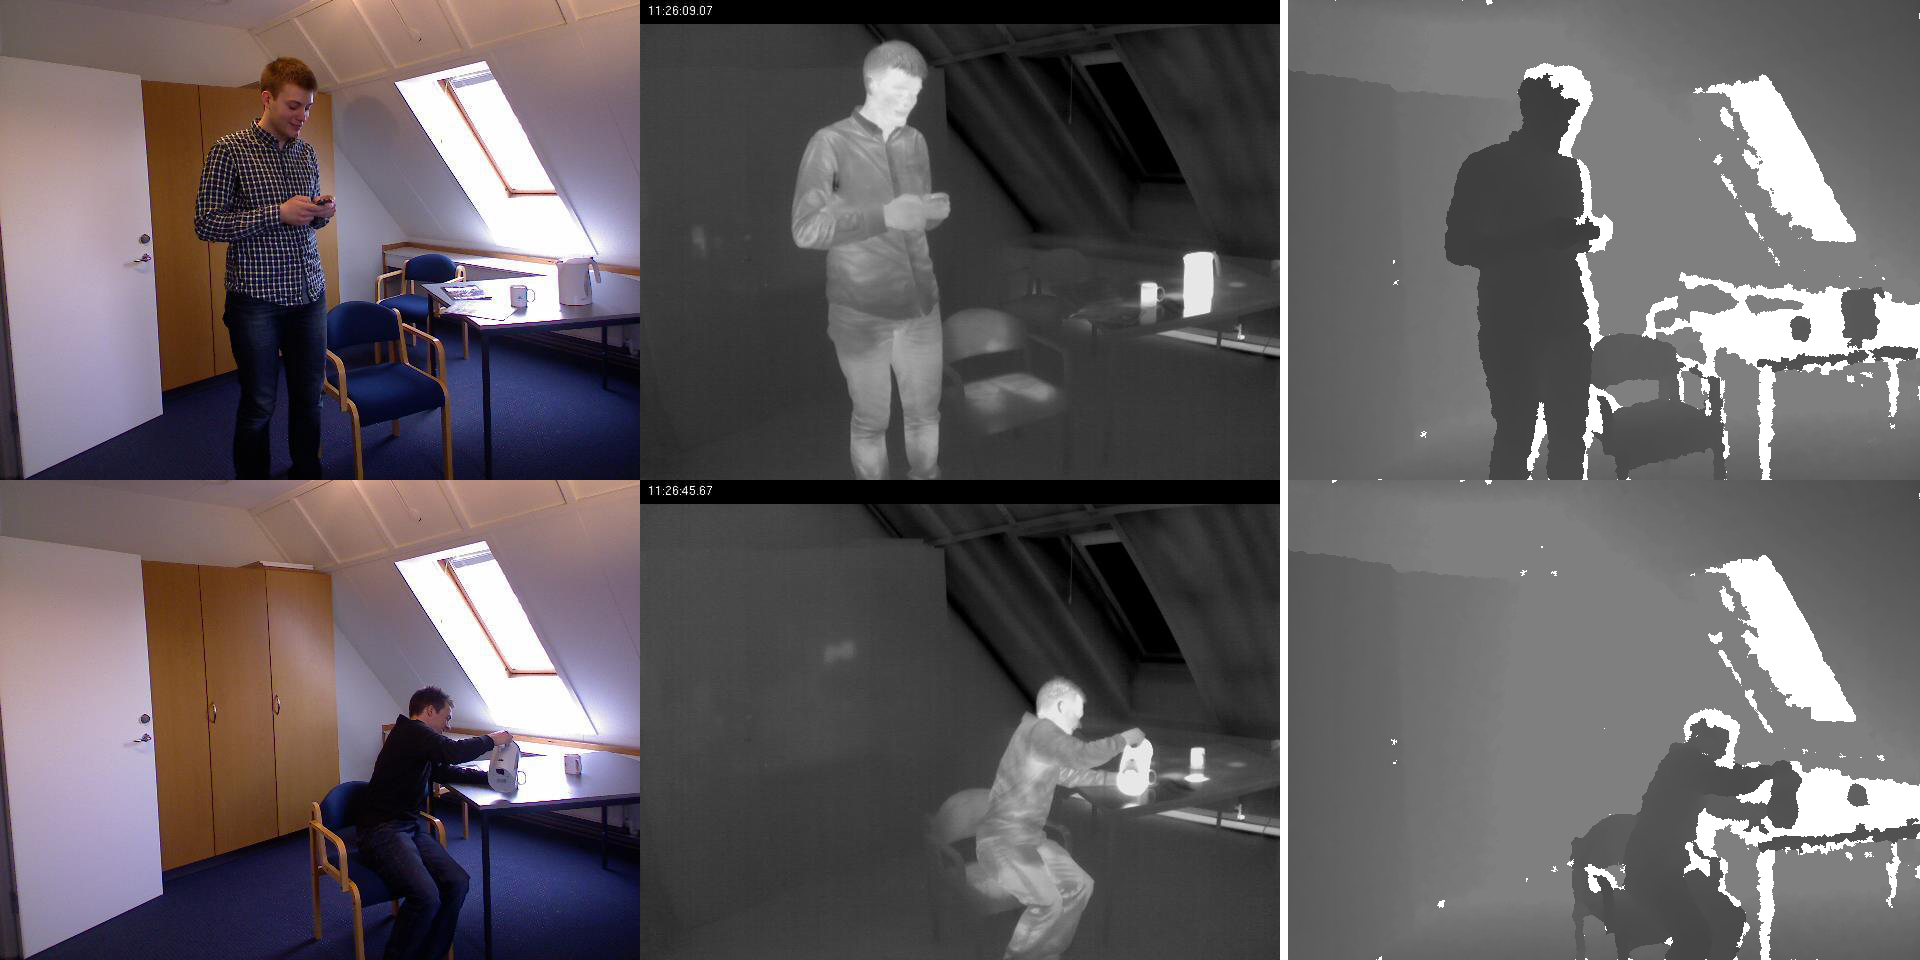
\includegraphics[width=0.48\textwidth]{Selection/2.png}
		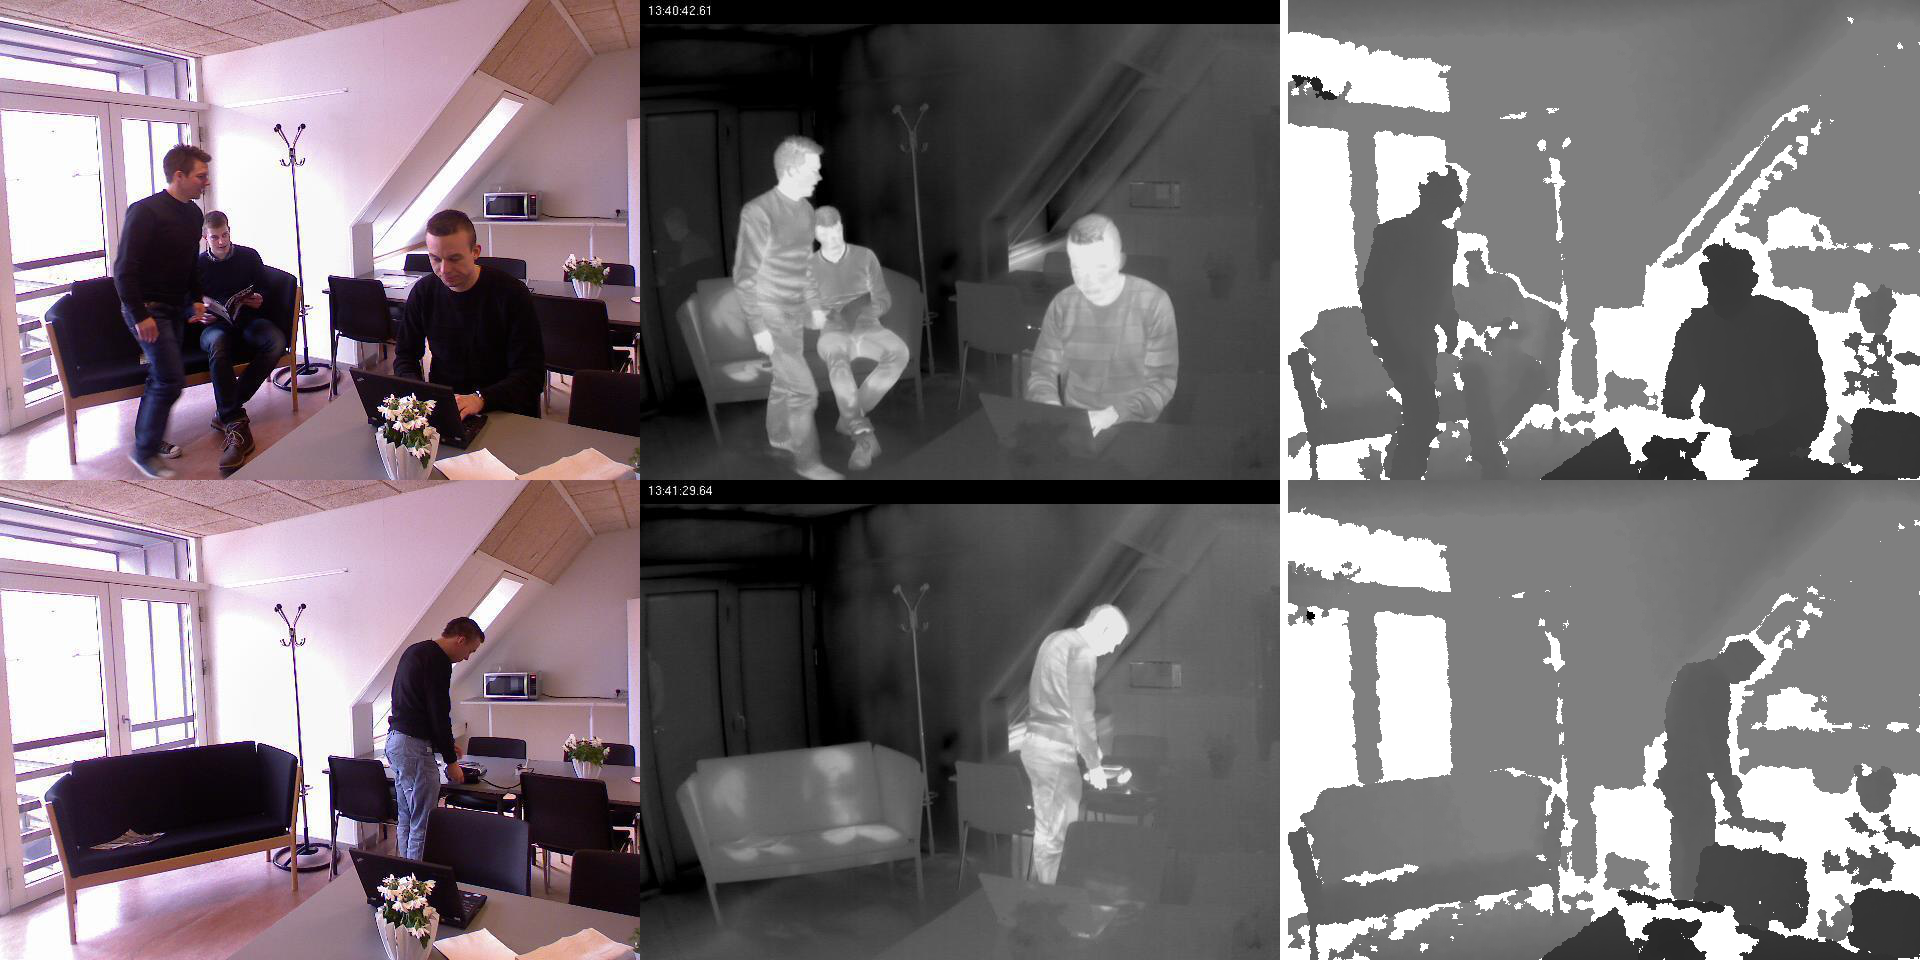
\includegraphics[width=0.48\textwidth]{Selection/3.png}
	\caption{Two views of each of the three scenes shown in the RGB, thermal, and depth modalities, respectively.}
	\label{fig:samplescenes}
\end{figure}

\begin{table}[htpb]
\centering
\begin{tabular}{llll}
\hline
Scene & Frames 	& Annotated frames 	& Depth range \\ \hline
1 		& 4693		& 1767	 						& 1-4 m \\
2 		& 2216		& 2016	 						& 1.4-1.9 m \\
3 		& 4628		& 1941	 						& 1-4 m \\ 
\hline
\end{tabular}
\caption{Annotated number of frames and spatial constraints of the scenes.}
\label{tab:scenes}
\end{table}

\subsection{Annotation}
%The frames are annotated using a pixel annotator tool ***ANDREAS TEXT HERE****
%
 %For each scene, human objects are annotated in the RGB modality. Each person is given a unique ID which he maintains throughout the scene. To obtain the corresponding masks in the thermal and depth modalities, the RGB masks are mapped using the registration algorithm of Section \ref{sec:registration}.
The acquired video was manually annotated frame-by-frame in a custom annotation program called Pixel Annotator. The dataset contains a large number of frames divided over a number of different sequences. All sequences have three modalities: RGB, depth, and thermal. The focus of the annotation has been on the persons in the scene and a mask-based annotation philosophy has been employed. That means that each person is covered by a mask and each mask (person) has a unique ID, which is consistent over frames. In this way the dataset can be used not only for background subtraction, but also for tracking and re-identification purposes. Since the main purpose of the dataset is background subtraction, a pixel-level annotation scheme was necessary - bounding boxes would not be sufficient.
 
As seen from Figure \ref{fig:pixelannotator}, Pixel Annotator provides a view of each modality with the current mask overlaid, as well as a raw view of the mask. It implements the registration algorithm described above so that the annotator can judge whether the mask fits in all modalities. Because the modalities are registered to each other, there is not specific masks for each modality, but a single mask for all.

\begin{figure}%
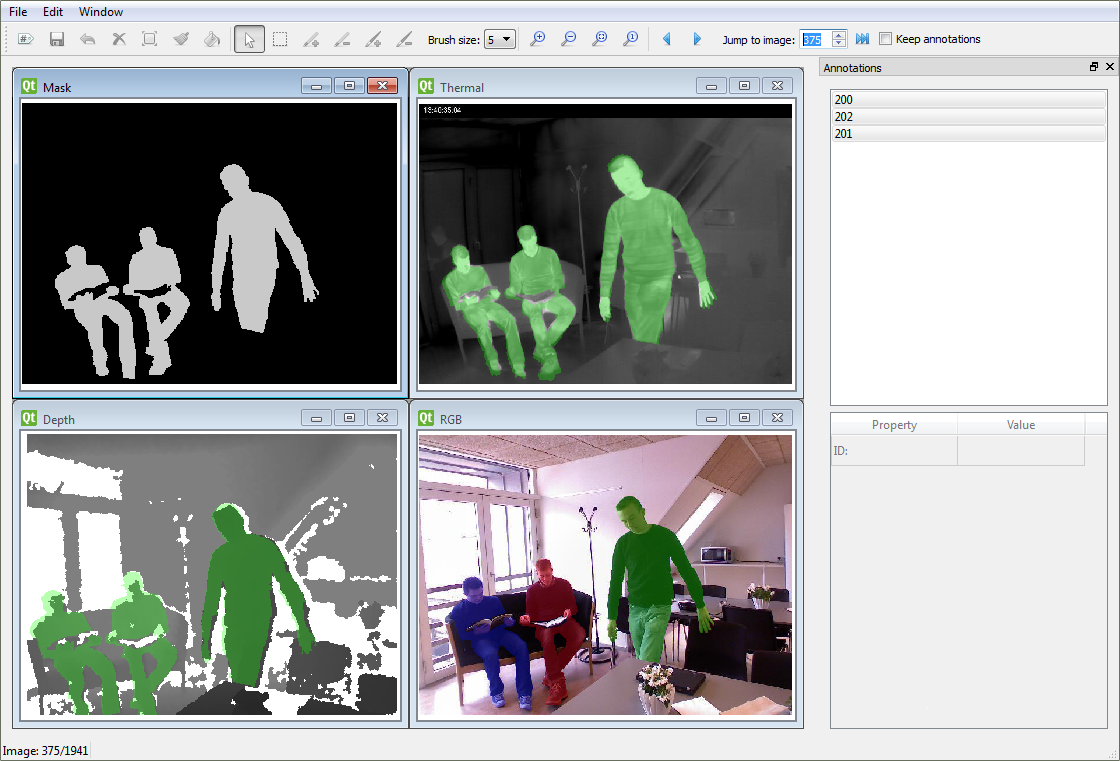
\includegraphics[width=0.48\textwidth]{pixelannotator2.png}%
\caption{Pixel Annotator showing the RGB masks and the corresponding, registered masks in the other views.}%
\label{fig:pixelannotator}%
\end{figure}

Each annotation can be initialized with an automatic segmentation using the GrabCut algorithm \cite{rother2004grabcut} to get quickly off the ground. Then Pixel Annotator provides pixel-wise editing functions to further refine the mask. Each annotation is associated with a numerical ID, and can have an arbitrary number of property fields associated with it. They can be boolean or contain strings, so advanced annotation can take place, all the way from simple occluded/not occluded fields to fields describing the current activity. Pixel Annotator is written in C++ on the Qt framework and is fully cross-platform compatible.

The data set and the registration algorithm is freely available at \cite{vapgroup}.

\subsection{Parameters and settings}
\label{ssec:parametersandsettings}

After some experiments regarding the use of Otsu's threshold in the background subtraction and generation of bounding boxes stage, we set $\sigma_\text{otsu} = 8.3$ for a connected component area of at least 0.1\% of the image, or  $\sigma_\text{otsu} = 12$ for other cases.

Since it is not possible to have a pixel-to-pixel correspondence among modalities, we define the correspondence at a grid cell level. The grids have been partitioned in $M \times N$ cells, being $M = 2$ and $N = 2$. The main idea of the grid partitioning is to reduce the variability of the regions in each GMM. At the same time, they are large enough to not condition the eventually computed overlap measure.

For the HOG descriptor, we defined: $H_\text{w} = 64 \times 128$, $H_\text{b} = 32 \times 32$, $H_\text{c}=16 \times 16$ and $H_{h} = 9$. The information of each cell is concatenated resulting in a vector of 36 values per block. This brings the final vector size of a grid cell to 4 blocks vertically $\times$ 2 blocks horizontally $\times$ 4 cells per block $\times$ 9 bins per cell $=$ 288 components. 

In order to compute the optical flow, and based on the tests performed in \cite{brkic2013combining}, we set the parameters of the given implementation according to the values that gave the best performance. In particular, the averaging window size was set to 2, the size of the pixel neighborhood considered when finding polynomial expansion in each pixel was set to 5 and the standard deviation of the Gaussian that is used to smooth derivatives used as a basis for the polynomial expansion to 1.1.  The remaining parameters were set to their default OpenCV values. For the HOOF descriptor, we defined $V_\text{b}$ = 8, to finally produce an 8-D feature vector.

For the depth descriptors, we defined $\theta_{I} = 8$ and $\phi_{G} = 8$.

For the thermal descriptors, we defined $T_{I} = 8$ and $T_{G} = 8$.

The parameter set up in the training of the GMMs is simply the number of mixtures, which have been set to a typical value of 3 mixture components.

\subsection{Experimental methodology and validation measures}
\label{ssec:validation}

The proposed baseline has been validated by means of a K-fold cross-validation (CV). The $R$ regions of interest have been divided in disjoint partitions, in which the cells' classifications and log-likelihoods' normalizations have been performed independently. In each iteration of the cross-validation, K-1 partitions are used to train the GMMs and the other one is used for testing, that is, each region of interest in the test set is predicted (at cell level) using models trained in an independent dataset (train set). Once all the regions in the $K$ different test partitions have been predicted, all the regions throughout the sequence of frames have been also predicted, and a final performance measure can be computed at frame level comparing the results of the predictions with the groundtruth, e.g. an overlap measure, explained below.

Moreover, in order to select the $\alpha$ and $\eta$ parameters for the individual prediction of the SM descriptor, a coarser-to-fine search strategy has been followed. The first coarse grid search is utilized to roughly estimate their value. In this search, a K-fold CV has tested $6 
\times 5$ combinations; $\alpha$ took the middle 6 of the 8 equidistant values in the range $[\mathrm{score}_{\mathrm{min}}, \mathrm{score}_{\mathrm{max}}]$ and $\eta$ the middle 5 of 7 equidistant values in the range $[0,1]$. Posteriorly, the fine search around the best coarse combination in each fold has been performed to find the best fine combination. A second K-fold CV tested the fine combinations, which consisted of a $7 \times 5$ grid centered in the corresponding best coarse combination. In this case the criterion to guide the search of the parameters selection is simply the subject detection accuracy, got comparing the result of the prediction to the ground truth.

Another coarse-to-fine grid search has been applied in order to select the SVM parameters $\gamma$ and $\zeta$. The coarse search is first used to identify a better region on the grid. For linear SVM, $\zeta$ is searched in the range $[2^{-5}, 2^{15}]$ in steps of $2^2$, that is, 11 values. RBF SVM uses in turn the same range of values for $\zeta$, whereas $\gamma$ is searched in the interval $[2^-13, 2^3]$ in steps of $2^2$, thus testing $11 \times 9$ combinations. After finding the best combination, a finer grid search on that region has been conducted, varying in $2^{1.5}$ in each direction centered on the value that produced the highest classification accuracy. Both procedures have been validated with K-fold CV, using the computed ground truth labels $t_{r}^m \in T$ to train the models. 

\begin{table}[h]\footnotesize
\center
\caption{Best cross-validation results for parameter selection of SVM models}
\label{table:svmgridsearch}
\begin{tabular}{|c|c|c|c|c|c|c|}
\cline{2-7} 
\multicolumn{1}{c|}{}&\multicolumn{3}{c|}{\textbf{Linear}}&\multicolumn{3}{c|}{\textbf{RBF}} \\
\hline
SVM Type & \gamma & \zeta & accuracy & \gamma & \zeta & accuracy \\ \hline
\textbf{Simple} & - & 45.2548 & 96.56 \% & 5.6569 & 22.6274 & 97.65   \% \\
\textbf{Stacked} & - & 1024 & 96.78 \% & 0.5 & 512 & 97.67  \% \\
\hline
  \end{tabular}
\end{table}

Lastly, we have used the Jaccard Index \cite{tan2002selecting}, also known as the Jaccard similarity coefficient, in order to compare the similarity between the groundtruth masks and the predicted masks in terms of overlap, thus assessing the performance of the proposed baseline. The degree of overlap between two binary sets $A$ and $B$ is computed as the ratio between the size of the intersection divided by the size of the union:
\begin{equation} \label{eq:jaccard}
overlap(A, B) = \frac{|A \cap B|}{|A \cup B|}
\end{equation}

This measure takes values in $[0,1]$, 0 meaning no overlap and 1 meaning perfect agreement between sets. $GT$ represents connected components of the ground truth binary masks, and $\hat{S}$ those of predicted binary masks from the different modalities individually or from the different fusion approaches. For each frame, the overlap is computed per person id and connected component, in such a way that connected components that have the same person id  or are connected in the ground truth constitute a set $A$, and they are compared to the blobs that coincide in the predicted binary masks, which constitute a set $B$. The overlap of each frame is then averaged by the number of sets found. It is therefore a pessimistic measure because a very tiny blob misclassified as a person in the predicted binary masks will account for 0 overlap, thus decreasing the mean overlap of the frame, so it can be considered as a lower bound on how accurate the prediction is. The final overlap is computed as the mean overlap of all frames having at least one blob, whether they be in the ground truth or in the predicted binary mask.

As commented in Section \ref{sect:bs}, the depth cue suffers from a halo effect around people or objects, thus complicating an accurate pixel-level segmentation at blob contours when applying background subtraction. This lack of accuracy is also caused by possible distortions, noise or other problems, and decreases the final overlap. Hence, a \emph{do not care region} (DCR) is often used. Such region is taken per frame by centering a morphology operator of different sizes at the ground truth binary masks blob contours and subtract it from those masks and from the predicted ones to compute the overlap. This way, we can compare the effect of using a growing DCR to the actual overlap.

\section{Experimental results}
\label{ssec:experimentalresults}

As explained in the last section, we assess the performance of the proposed baseline using the Jaccard overlap measure (Eq. \ref{eq:jaccard}). Figure \ref{fig:overlapgraph} depicts the obtained overlap for individual predictions and fusion predictions with different fusion approaches. Tables \ref{table:individual} and \ref{table:linearstacked} are included to compare the differences between using the descriptors separately and after fusing them. Notice that in plots showing fusion results, only two cases are considered, owing to color and depth modalities share the same original $FG$ masks.

\begin{table}[h]\footnotesize
\center
\caption{Overlap results of the individual predictions for each description}
\label{table:individual}
\begin{tabular}{|l|l|l|l|l|l|}
\hline
&\textbf{HOG}&\textbf{SM}&\textbf{HOOF}&\textbf{HIOG}&\textbf{HON}\\\hline
\textbf{0}&62.10 \% &63.12 \%&56.97 \%&46.35 \%&56.76 \%\\\hline
\textbf{1}&64.71 \%&65.85 \%&59.41 \%&47.99 \%&59.09 \%\\\hline
\textbf{3}&67.59 \%&69.02 \%&62.13 \%&50.85 \%&61.70 \%\\\hline
\textbf{5}&68.65 \%&70.40 \%&63.20 \%&53.02 \%&62.77 \%\\\hline
\textbf{7}&68.65 \%&70.72 \%&63.28 \%&54.45 \%&62.94 \%\\\hline
\end{tabular}
\end{table}


\begin{table}[h]\footnotesize
\center
\caption{Overlap results of fusion using Stacked Linear SVM for each modality}
\label{table:linearstacked}
\begin{tabular}{|c|c|c|}
\hline
\textbf{DCR}&\textbf{Thermal}&\textbf{Color/Depth}\\\hline
\textbf{0}&49.64 \%&64.65 \%\\\hline
\textbf{1}&51.33 \%&67.39 \%\\\hline
\textbf{3}&54.29 \%&70.43 \%\\\hline
\textbf{5}&56.56 \%&71.58 \%\\\hline
\textbf{7}&58.11 \%&71.63 \%\\\hline
\end{tabular}
\end{table}

%Linear SVM is used as baseline classifier. It offers good performance relative to other linear classifiers and %fast to run.


 \begin{figure}[H]
	 \centering
	 \begin{subfigure}[b]{0.47\textwidth}
 		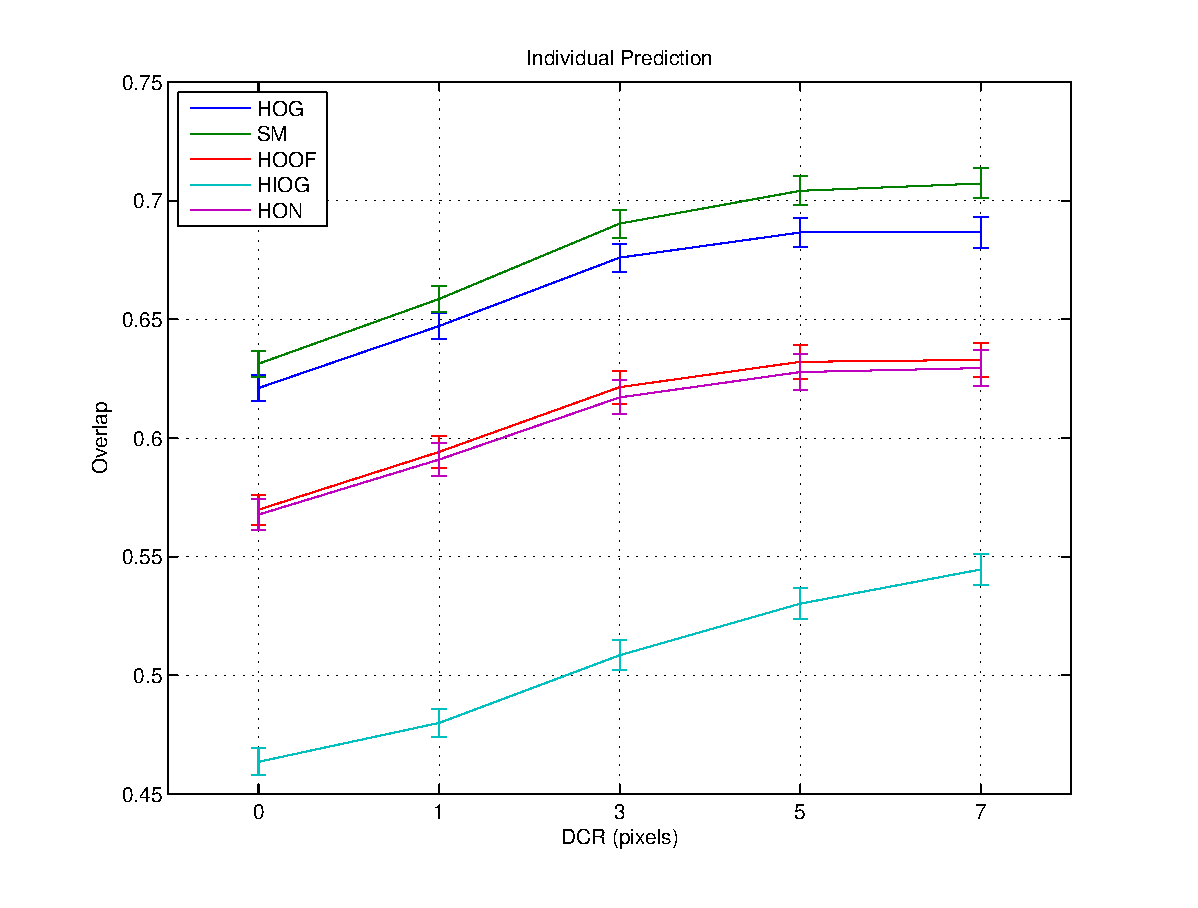
\includegraphics[width=1\textwidth]{results/individualprediction.eps}
 		\caption{Individual prediction}
    		\label{fig:individualprediction}
 	\end{subfigure}
	 ~
	\begin{subfigure}[b]{0.47\textwidth}
 		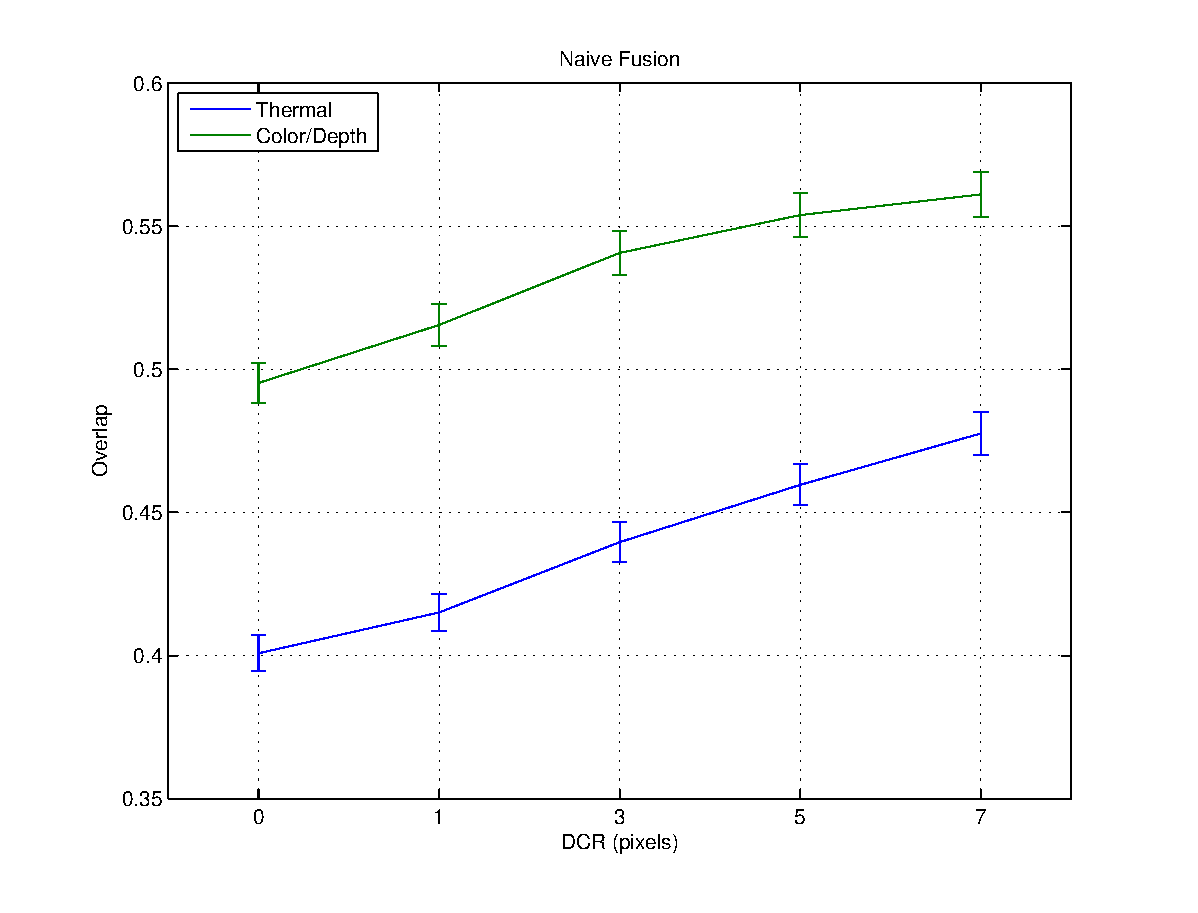
\includegraphics[width=1\textwidth]{results/naivefusion.eps}
 		\caption{Naive fusion}
    		\label{fig:naivefusion}
 	\end{subfigure}
	 \\
	\begin{subfigure}[b]{0.47\textwidth}
 		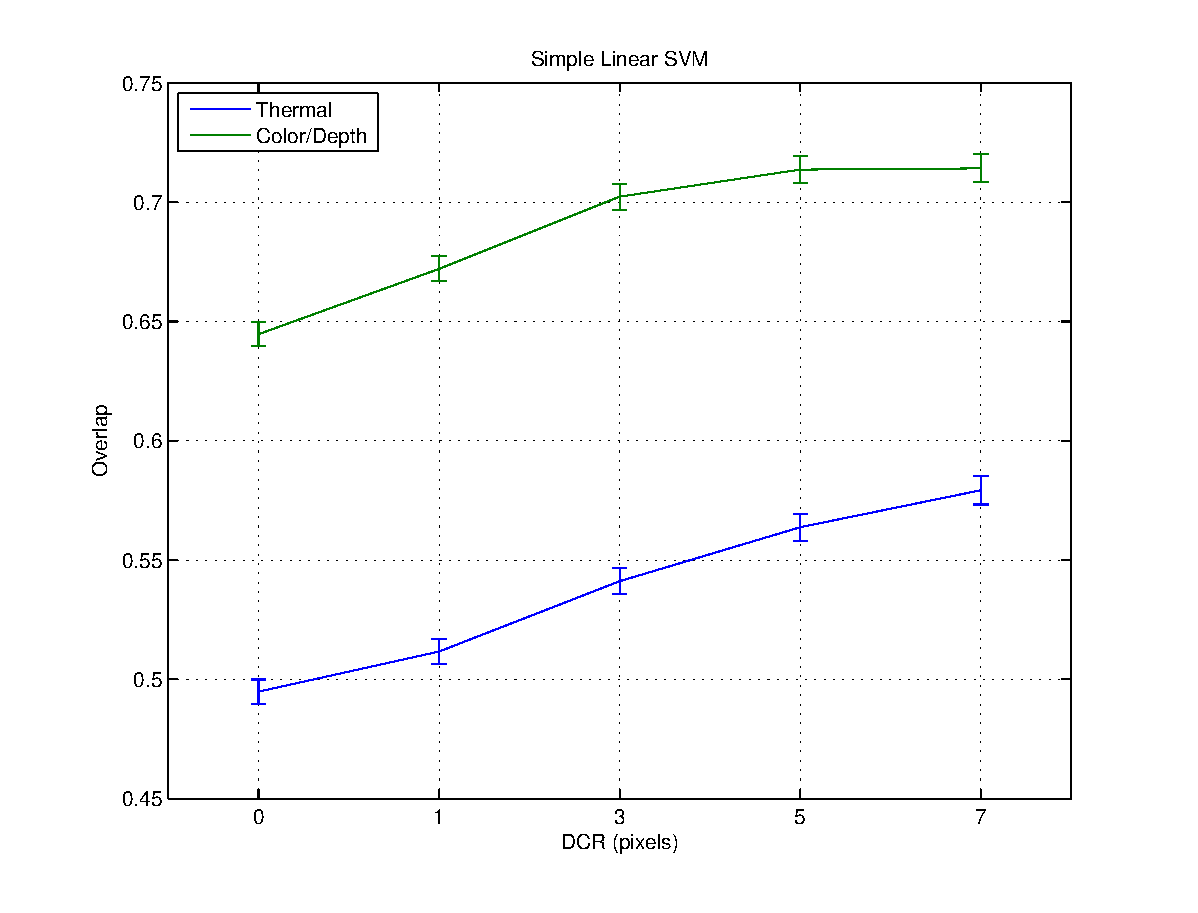
\includegraphics[width=1\textwidth]{results/simplelinearsvm.eps} 			
		\caption{Fusion using Simple linear SVM}
    		\label{fig:simplelinearsvm}
 	\end{subfigure}
	~
	\begin{subfigure}[b]{0.47\textwidth}
 		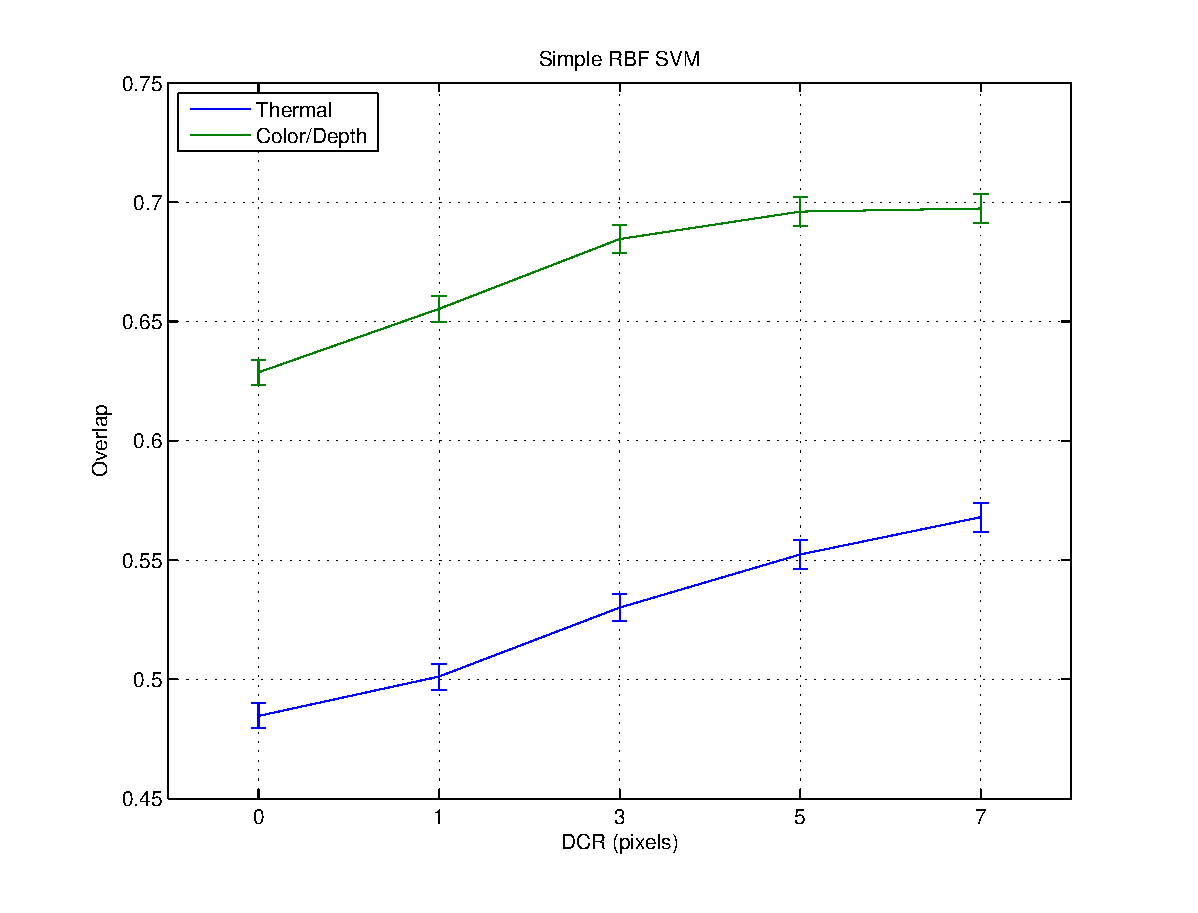
\includegraphics[width=1\textwidth]{results/simplerbfsvm.eps} 			
		\caption{Fusion using Simple RBF SVM}
    		\label{fig:simplerbfsvm}
 	\end{subfigure}
	\\
	\begin{subfigure}[b]{0.47\textwidth}
 		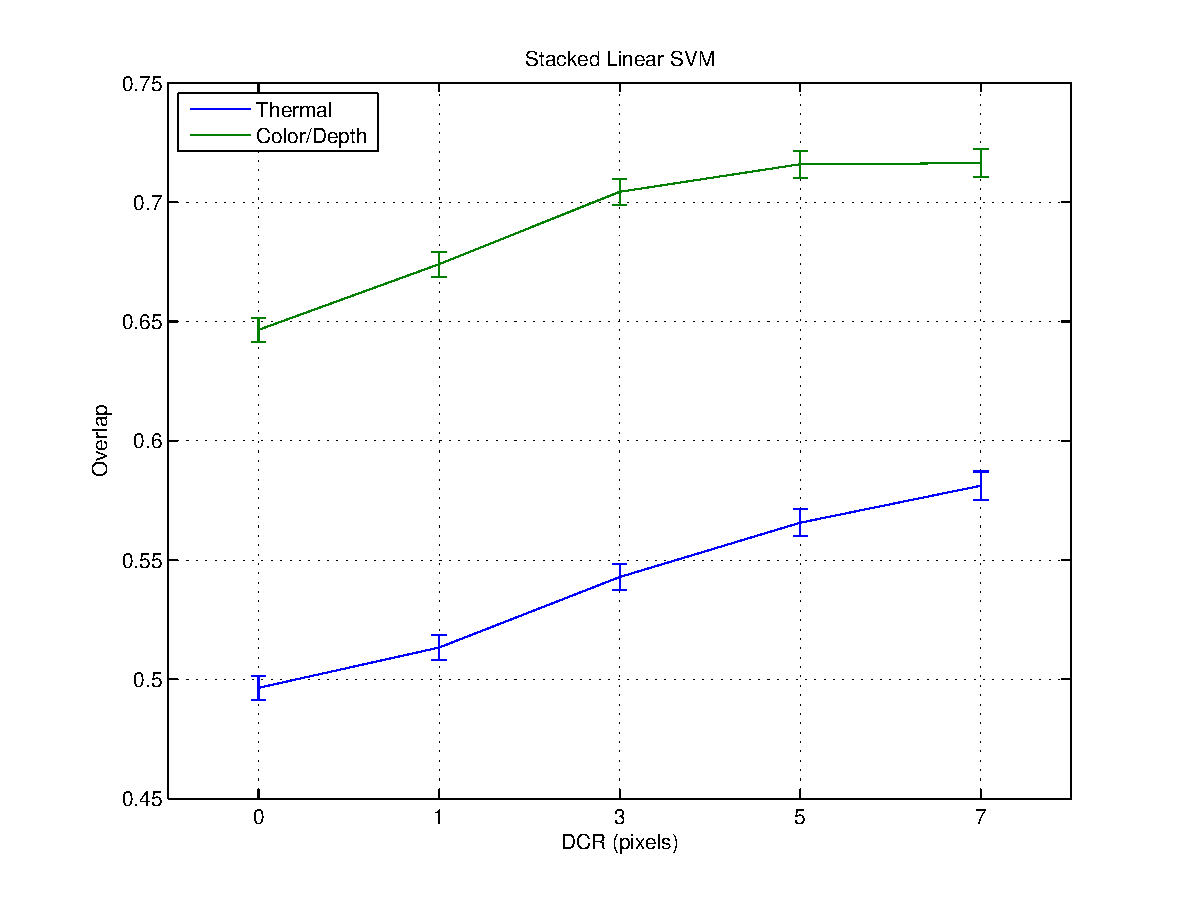
\includegraphics[width=1\textwidth]{results/stackedlinearsvm.eps} 			
		\caption{Fusion using Stacked Linear SVM}
    		\label{fig:stackedlinearsvm}
 	\end{subfigure}
	~
	\begin{subfigure}[b]{0.47\textwidth}
 		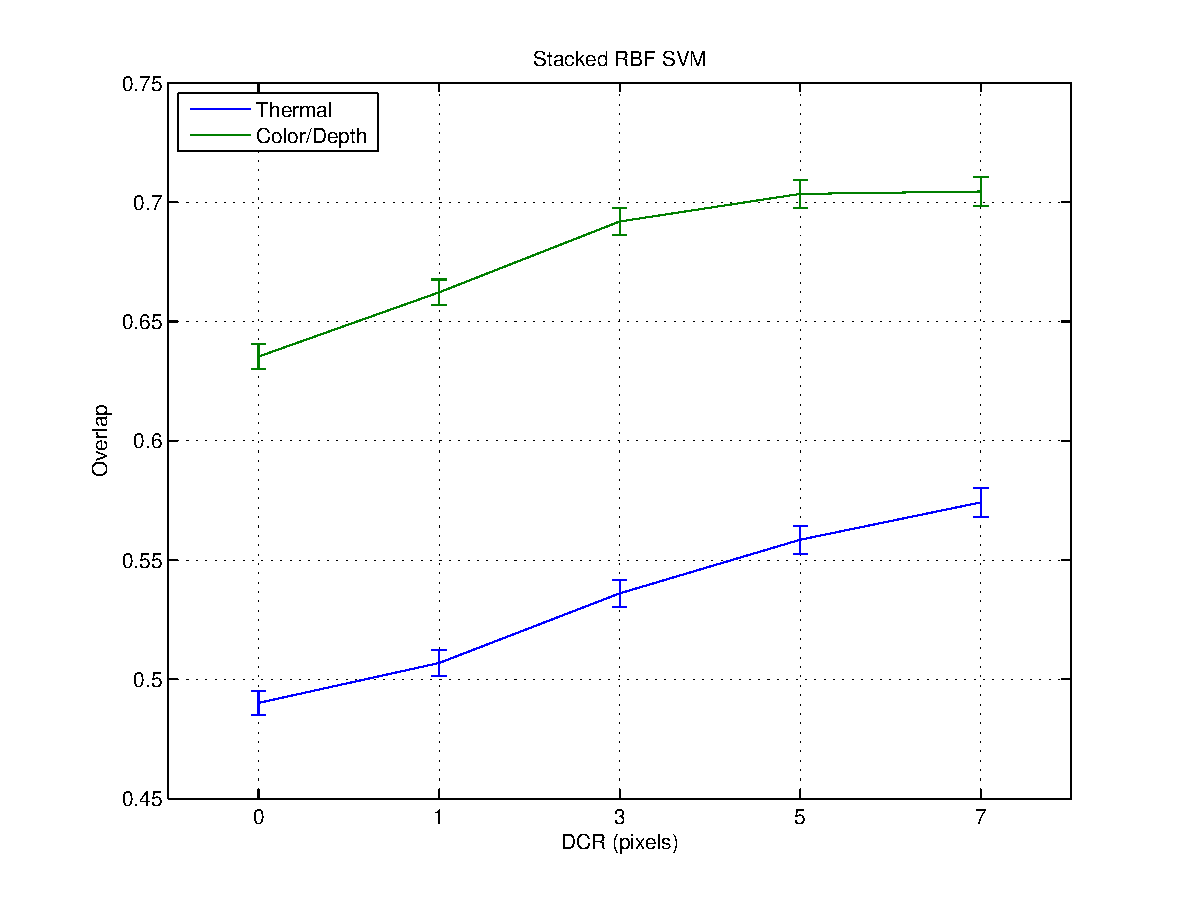
\includegraphics[width=1\textwidth]{results/stackedrbfsvm.eps} 			
		\caption{Fusion using Stacked RBF SVM}
    		\label{fig:stackedrbfsvm}
 	\end{subfigure}
	\caption{Overlap results for the different individual and fusion prediction approaches.}
	\label{fig:overlapgraph}
\end{figure}


{\small
\bibliographystyle{ieee}
\bibliography{references}
}

\end{document}
